
\documentclass{article} % For LaTeX2e
\usepackage{iclr2021_conference,times}

% Optional math commands from https://github.com/goodfeli/dlbook_notation.
%%%%% NEW MATH DEFINITIONS %%%%%

\usepackage{amsmath,amsfonts,bm}

% Mark sections of captions for referring to divisions of figures
\newcommand{\figleft}{{\em (Left)}}
\newcommand{\figcenter}{{\em (Center)}}
\newcommand{\figright}{{\em (Right)}}
\newcommand{\figtop}{{\em (Top)}}
\newcommand{\figbottom}{{\em (Bottom)}}
\newcommand{\captiona}{{\em (a)}}
\newcommand{\captionb}{{\em (b)}}
\newcommand{\captionc}{{\em (c)}}
\newcommand{\captiond}{{\em (d)}}

% Highlight a newly defined term
\newcommand{\newterm}[1]{{\bf #1}}


% Figure reference, lower-case.
\def\figref#1{figure~\ref{#1}}
% Figure reference, capital. For start of sentence
\def\Figref#1{Figure~\ref{#1}}
\def\twofigref#1#2{figures \ref{#1} and \ref{#2}}
\def\quadfigref#1#2#3#4{figures \ref{#1}, \ref{#2}, \ref{#3} and \ref{#4}}
% Section reference, lower-case.
\def\secref#1{section~\ref{#1}}
% Section reference, capital.
\def\Secref#1{Section~\ref{#1}}
% Reference to two sections.
\def\twosecrefs#1#2{sections \ref{#1} and \ref{#2}}
% Reference to three sections.
\def\secrefs#1#2#3{sections \ref{#1}, \ref{#2} and \ref{#3}}
% Reference to an equation, lower-case.
\def\eqref#1{equation~\ref{#1}}
% Reference to an equation, upper case
\def\Eqref#1{Equation~\ref{#1}}
% A raw reference to an equation---avoid using if possible
\def\plaineqref#1{\ref{#1}}
% Reference to a chapter, lower-case.
\def\chapref#1{chapter~\ref{#1}}
% Reference to an equation, upper case.
\def\Chapref#1{Chapter~\ref{#1}}
% Reference to a range of chapters
\def\rangechapref#1#2{chapters\ref{#1}--\ref{#2}}
% Reference to an algorithm, lower-case.
\def\algref#1{algorithm~\ref{#1}}
% Reference to an algorithm, upper case.
\def\Algref#1{Algorithm~\ref{#1}}
\def\twoalgref#1#2{algorithms \ref{#1} and \ref{#2}}
\def\Twoalgref#1#2{Algorithms \ref{#1} and \ref{#2}}
% Reference to a part, lower case
\def\partref#1{part~\ref{#1}}
% Reference to a part, upper case
\def\Partref#1{Part~\ref{#1}}
\def\twopartref#1#2{parts \ref{#1} and \ref{#2}}

\def\ceil#1{\lceil #1 \rceil}
\def\floor#1{\lfloor #1 \rfloor}
\def\1{\bm{1}}
\newcommand{\train}{\mathcal{D}}
\newcommand{\valid}{\mathcal{D_{\mathrm{valid}}}}
\newcommand{\test}{\mathcal{D_{\mathrm{test}}}}

\def\eps{{\epsilon}}


% Random variables
\def\reta{{\textnormal{$\eta$}}}
\def\ra{{\textnormal{a}}}
\def\rb{{\textnormal{b}}}
\def\rc{{\textnormal{c}}}
\def\rd{{\textnormal{d}}}
\def\re{{\textnormal{e}}}
\def\rf{{\textnormal{f}}}
\def\rg{{\textnormal{g}}}
\def\rh{{\textnormal{h}}}
\def\ri{{\textnormal{i}}}
\def\rj{{\textnormal{j}}}
\def\rk{{\textnormal{k}}}
\def\rl{{\textnormal{l}}}
% rm is already a command, just don't name any random variables m
\def\rn{{\textnormal{n}}}
\def\ro{{\textnormal{o}}}
\def\rp{{\textnormal{p}}}
\def\rq{{\textnormal{q}}}
\def\rr{{\textnormal{r}}}
\def\rs{{\textnormal{s}}}
\def\rt{{\textnormal{t}}}
\def\ru{{\textnormal{u}}}
\def\rv{{\textnormal{v}}}
\def\rw{{\textnormal{w}}}
\def\rx{{\textnormal{x}}}
\def\ry{{\textnormal{y}}}
\def\rz{{\textnormal{z}}}

% Random vectors
\def\rvepsilon{{\mathbf{\epsilon}}}
\def\rvtheta{{\mathbf{\theta}}}
\def\rva{{\mathbf{a}}}
\def\rvb{{\mathbf{b}}}
\def\rvc{{\mathbf{c}}}
\def\rvd{{\mathbf{d}}}
\def\rve{{\mathbf{e}}}
\def\rvf{{\mathbf{f}}}
\def\rvg{{\mathbf{g}}}
\def\rvh{{\mathbf{h}}}
\def\rvu{{\mathbf{i}}}
\def\rvj{{\mathbf{j}}}
\def\rvk{{\mathbf{k}}}
\def\rvl{{\mathbf{l}}}
\def\rvm{{\mathbf{m}}}
\def\rvn{{\mathbf{n}}}
\def\rvo{{\mathbf{o}}}
\def\rvp{{\mathbf{p}}}
\def\rvq{{\mathbf{q}}}
\def\rvr{{\mathbf{r}}}
\def\rvs{{\mathbf{s}}}
\def\rvt{{\mathbf{t}}}
\def\rvu{{\mathbf{u}}}
\def\rvv{{\mathbf{v}}}
\def\rvw{{\mathbf{w}}}
\def\rvx{{\mathbf{x}}}
\def\rvy{{\mathbf{y}}}
\def\rvz{{\mathbf{z}}}

% Elements of random vectors
\def\erva{{\textnormal{a}}}
\def\ervb{{\textnormal{b}}}
\def\ervc{{\textnormal{c}}}
\def\ervd{{\textnormal{d}}}
\def\erve{{\textnormal{e}}}
\def\ervf{{\textnormal{f}}}
\def\ervg{{\textnormal{g}}}
\def\ervh{{\textnormal{h}}}
\def\ervi{{\textnormal{i}}}
\def\ervj{{\textnormal{j}}}
\def\ervk{{\textnormal{k}}}
\def\ervl{{\textnormal{l}}}
\def\ervm{{\textnormal{m}}}
\def\ervn{{\textnormal{n}}}
\def\ervo{{\textnormal{o}}}
\def\ervp{{\textnormal{p}}}
\def\ervq{{\textnormal{q}}}
\def\ervr{{\textnormal{r}}}
\def\ervs{{\textnormal{s}}}
\def\ervt{{\textnormal{t}}}
\def\ervu{{\textnormal{u}}}
\def\ervv{{\textnormal{v}}}
\def\ervw{{\textnormal{w}}}
\def\ervx{{\textnormal{x}}}
\def\ervy{{\textnormal{y}}}
\def\ervz{{\textnormal{z}}}

% Random matrices
\def\rmA{{\mathbf{A}}}
\def\rmB{{\mathbf{B}}}
\def\rmC{{\mathbf{C}}}
\def\rmD{{\mathbf{D}}}
\def\rmE{{\mathbf{E}}}
\def\rmF{{\mathbf{F}}}
\def\rmG{{\mathbf{G}}}
\def\rmH{{\mathbf{H}}}
\def\rmI{{\mathbf{I}}}
\def\rmJ{{\mathbf{J}}}
\def\rmK{{\mathbf{K}}}
\def\rmL{{\mathbf{L}}}
\def\rmM{{\mathbf{M}}}
\def\rmN{{\mathbf{N}}}
\def\rmO{{\mathbf{O}}}
\def\rmP{{\mathbf{P}}}
\def\rmQ{{\mathbf{Q}}}
\def\rmR{{\mathbf{R}}}
\def\rmS{{\mathbf{S}}}
\def\rmT{{\mathbf{T}}}
\def\rmU{{\mathbf{U}}}
\def\rmV{{\mathbf{V}}}
\def\rmW{{\mathbf{W}}}
\def\rmX{{\mathbf{X}}}
\def\rmY{{\mathbf{Y}}}
\def\rmZ{{\mathbf{Z}}}

% Elements of random matrices
\def\ermA{{\textnormal{A}}}
\def\ermB{{\textnormal{B}}}
\def\ermC{{\textnormal{C}}}
\def\ermD{{\textnormal{D}}}
\def\ermE{{\textnormal{E}}}
\def\ermF{{\textnormal{F}}}
\def\ermG{{\textnormal{G}}}
\def\ermH{{\textnormal{H}}}
\def\ermI{{\textnormal{I}}}
\def\ermJ{{\textnormal{J}}}
\def\ermK{{\textnormal{K}}}
\def\ermL{{\textnormal{L}}}
\def\ermM{{\textnormal{M}}}
\def\ermN{{\textnormal{N}}}
\def\ermO{{\textnormal{O}}}
\def\ermP{{\textnormal{P}}}
\def\ermQ{{\textnormal{Q}}}
\def\ermR{{\textnormal{R}}}
\def\ermS{{\textnormal{S}}}
\def\ermT{{\textnormal{T}}}
\def\ermU{{\textnormal{U}}}
\def\ermV{{\textnormal{V}}}
\def\ermW{{\textnormal{W}}}
\def\ermX{{\textnormal{X}}}
\def\ermY{{\textnormal{Y}}}
\def\ermZ{{\textnormal{Z}}}

% Vectors
\def\vzero{{\bm{0}}}
\def\vone{{\bm{1}}}
\def\vmu{{\bm{\mu}}}
\def\vtheta{{\bm{\theta}}}
\def\va{{\bm{a}}}
\def\vb{{\bm{b}}}
\def\vc{{\bm{c}}}
\def\vd{{\bm{d}}}
\def\ve{{\bm{e}}}
\def\vf{{\bm{f}}}
\def\vg{{\bm{g}}}
\def\vh{{\bm{h}}}
\def\vi{{\bm{i}}}
\def\vj{{\bm{j}}}
\def\vk{{\bm{k}}}
\def\vl{{\bm{l}}}
\def\vm{{\bm{m}}}
\def\vn{{\bm{n}}}
\def\vo{{\bm{o}}}
\def\vp{{\bm{p}}}
\def\vq{{\bm{q}}}
\def\vr{{\bm{r}}}
\def\vs{{\bm{s}}}
\def\vt{{\bm{t}}}
\def\vu{{\bm{u}}}
\def\vv{{\bm{v}}}
\def\vw{{\bm{w}}}
\def\vx{{\bm{x}}}
\def\vy{{\bm{y}}}
\def\vz{{\bm{z}}}

% Elements of vectors
\def\evalpha{{\alpha}}
\def\evbeta{{\beta}}
\def\evepsilon{{\epsilon}}
\def\evlambda{{\lambda}}
\def\evomega{{\omega}}
\def\evmu{{\mu}}
\def\evpsi{{\psi}}
\def\evsigma{{\sigma}}
\def\evtheta{{\theta}}
\def\eva{{a}}
\def\evb{{b}}
\def\evc{{c}}
\def\evd{{d}}
\def\eve{{e}}
\def\evf{{f}}
\def\evg{{g}}
\def\evh{{h}}
\def\evi{{i}}
\def\evj{{j}}
\def\evk{{k}}
\def\evl{{l}}
\def\evm{{m}}
\def\evn{{n}}
\def\evo{{o}}
\def\evp{{p}}
\def\evq{{q}}
\def\evr{{r}}
\def\evs{{s}}
\def\evt{{t}}
\def\evu{{u}}
\def\evv{{v}}
\def\evw{{w}}
\def\evx{{x}}
\def\evy{{y}}
\def\evz{{z}}

% Matrix
\def\mA{{\bm{A}}}
\def\mB{{\bm{B}}}
\def\mC{{\bm{C}}}
\def\mD{{\bm{D}}}
\def\mE{{\bm{E}}}
\def\mF{{\bm{F}}}
\def\mG{{\bm{G}}}
\def\mH{{\bm{H}}}
\def\mI{{\bm{I}}}
\def\mJ{{\bm{J}}}
\def\mK{{\bm{K}}}
\def\mL{{\bm{L}}}
\def\mM{{\bm{M}}}
\def\mN{{\bm{N}}}
\def\mO{{\bm{O}}}
\def\mP{{\bm{P}}}
\def\mQ{{\bm{Q}}}
\def\mR{{\bm{R}}}
\def\mS{{\bm{S}}}
\def\mT{{\bm{T}}}
\def\mU{{\bm{U}}}
\def\mV{{\bm{V}}}
\def\mW{{\bm{W}}}
\def\mX{{\bm{X}}}
\def\mY{{\bm{Y}}}
\def\mZ{{\bm{Z}}}
\def\mBeta{{\bm{\beta}}}
\def\mPhi{{\bm{\Phi}}}
\def\mLambda{{\bm{\Lambda}}}
\def\mSigma{{\bm{\Sigma}}}

% Tensor
\DeclareMathAlphabet{\mathsfit}{\encodingdefault}{\sfdefault}{m}{sl}
\SetMathAlphabet{\mathsfit}{bold}{\encodingdefault}{\sfdefault}{bx}{n}
\newcommand{\tens}[1]{\bm{\mathsfit{#1}}}
\def\tA{{\tens{A}}}
\def\tB{{\tens{B}}}
\def\tC{{\tens{C}}}
\def\tD{{\tens{D}}}
\def\tE{{\tens{E}}}
\def\tF{{\tens{F}}}
\def\tG{{\tens{G}}}
\def\tH{{\tens{H}}}
\def\tI{{\tens{I}}}
\def\tJ{{\tens{J}}}
\def\tK{{\tens{K}}}
\def\tL{{\tens{L}}}
\def\tM{{\tens{M}}}
\def\tN{{\tens{N}}}
\def\tO{{\tens{O}}}
\def\tP{{\tens{P}}}
\def\tQ{{\tens{Q}}}
\def\tR{{\tens{R}}}
\def\tS{{\tens{S}}}
\def\tT{{\tens{T}}}
\def\tU{{\tens{U}}}
\def\tV{{\tens{V}}}
\def\tW{{\tens{W}}}
\def\tX{{\tens{X}}}
\def\tY{{\tens{Y}}}
\def\tZ{{\tens{Z}}}


% Graph
\def\gA{{\mathcal{A}}}
\def\gB{{\mathcal{B}}}
\def\gC{{\mathcal{C}}}
\def\gD{{\mathcal{D}}}
\def\gE{{\mathcal{E}}}
\def\gF{{\mathcal{F}}}
\def\gG{{\mathcal{G}}}
\def\gH{{\mathcal{H}}}
\def\gI{{\mathcal{I}}}
\def\gJ{{\mathcal{J}}}
\def\gK{{\mathcal{K}}}
\def\gL{{\mathcal{L}}}
\def\gM{{\mathcal{M}}}
\def\gN{{\mathcal{N}}}
\def\gO{{\mathcal{O}}}
\def\gP{{\mathcal{P}}}
\def\gQ{{\mathcal{Q}}}
\def\gR{{\mathcal{R}}}
\def\gS{{\mathcal{S}}}
\def\gT{{\mathcal{T}}}
\def\gU{{\mathcal{U}}}
\def\gV{{\mathcal{V}}}
\def\gW{{\mathcal{W}}}
\def\gX{{\mathcal{X}}}
\def\gY{{\mathcal{Y}}}
\def\gZ{{\mathcal{Z}}}

% Sets
\def\sA{{\mathbb{A}}}
\def\sB{{\mathbb{B}}}
\def\sC{{\mathbb{C}}}
\def\sD{{\mathbb{D}}}
% Don't use a set called E, because this would be the same as our symbol
% for expectation.
\def\sF{{\mathbb{F}}}
\def\sG{{\mathbb{G}}}
\def\sH{{\mathbb{H}}}
\def\sI{{\mathbb{I}}}
\def\sJ{{\mathbb{J}}}
\def\sK{{\mathbb{K}}}
\def\sL{{\mathbb{L}}}
\def\sM{{\mathbb{M}}}
\def\sN{{\mathbb{N}}}
\def\sO{{\mathbb{O}}}
\def\sP{{\mathbb{P}}}
\def\sQ{{\mathbb{Q}}}
\def\sR{{\mathbb{R}}}
\def\sS{{\mathbb{S}}}
\def\sT{{\mathbb{T}}}
\def\sU{{\mathbb{U}}}
\def\sV{{\mathbb{V}}}
\def\sW{{\mathbb{W}}}
\def\sX{{\mathbb{X}}}
\def\sY{{\mathbb{Y}}}
\def\sZ{{\mathbb{Z}}}

% Entries of a matrix
\def\emLambda{{\Lambda}}
\def\emA{{A}}
\def\emB{{B}}
\def\emC{{C}}
\def\emD{{D}}
\def\emE{{E}}
\def\emF{{F}}
\def\emG{{G}}
\def\emH{{H}}
\def\emI{{I}}
\def\emJ{{J}}
\def\emK{{K}}
\def\emL{{L}}
\def\emM{{M}}
\def\emN{{N}}
\def\emO{{O}}
\def\emP{{P}}
\def\emQ{{Q}}
\def\emR{{R}}
\def\emS{{S}}
\def\emT{{T}}
\def\emU{{U}}
\def\emV{{V}}
\def\emW{{W}}
\def\emX{{X}}
\def\emY{{Y}}
\def\emZ{{Z}}
\def\emSigma{{\Sigma}}

% entries of a tensor
% Same font as tensor, without \bm wrapper
\newcommand{\etens}[1]{\mathsfit{#1}}
\def\etLambda{{\etens{\Lambda}}}
\def\etA{{\etens{A}}}
\def\etB{{\etens{B}}}
\def\etC{{\etens{C}}}
\def\etD{{\etens{D}}}
\def\etE{{\etens{E}}}
\def\etF{{\etens{F}}}
\def\etG{{\etens{G}}}
\def\etH{{\etens{H}}}
\def\etI{{\etens{I}}}
\def\etJ{{\etens{J}}}
\def\etK{{\etens{K}}}
\def\etL{{\etens{L}}}
\def\etM{{\etens{M}}}
\def\etN{{\etens{N}}}
\def\etO{{\etens{O}}}
\def\etP{{\etens{P}}}
\def\etQ{{\etens{Q}}}
\def\etR{{\etens{R}}}
\def\etS{{\etens{S}}}
\def\etT{{\etens{T}}}
\def\etU{{\etens{U}}}
\def\etV{{\etens{V}}}
\def\etW{{\etens{W}}}
\def\etX{{\etens{X}}}
\def\etY{{\etens{Y}}}
\def\etZ{{\etens{Z}}}

% The true underlying data generating distribution
\newcommand{\pdata}{p_{\rm{data}}}
% The empirical distribution defined by the training set
\newcommand{\ptrain}{\hat{p}_{\rm{data}}}
\newcommand{\Ptrain}{\hat{P}_{\rm{data}}}
% The model distribution
\newcommand{\pmodel}{p_{\rm{model}}}
\newcommand{\Pmodel}{P_{\rm{model}}}
\newcommand{\ptildemodel}{\tilde{p}_{\rm{model}}}
% Stochastic autoencoder distributions
\newcommand{\pencode}{p_{\rm{encoder}}}
\newcommand{\pdecode}{p_{\rm{decoder}}}
\newcommand{\precons}{p_{\rm{reconstruct}}}

\newcommand{\laplace}{\mathrm{Laplace}} % Laplace distribution

\newcommand{\E}{\mathbb{E}}
\newcommand{\Ls}{\mathcal{L}}
\newcommand{\R}{\mathbb{R}}
\newcommand{\emp}{\tilde{p}}
\newcommand{\lr}{\alpha}
\newcommand{\reg}{\lambda}
\newcommand{\rect}{\mathrm{rectifier}}
\newcommand{\softmax}{\mathrm{softmax}}
\newcommand{\sigmoid}{\sigma}
\newcommand{\softplus}{\zeta}
\newcommand{\KL}{D_{\mathrm{KL}}}
\newcommand{\Var}{\mathrm{Var}}
\newcommand{\standarderror}{\mathrm{SE}}
\newcommand{\Cov}{\mathrm{Cov}}
% Wolfram Mathworld says $L^2$ is for function spaces and $\ell^2$ is for vectors
% But then they seem to use $L^2$ for vectors throughout the site, and so does
% wikipedia.
\newcommand{\normlzero}{L^0}
\newcommand{\normlone}{L^1}
\newcommand{\normltwo}{L^2}
\newcommand{\normlp}{L^p}
\newcommand{\normmax}{L^\infty}

\newcommand{\parents}{Pa} % See usage in notation.tex. Chosen to match Daphne's book.

\DeclareMathOperator*{\argmax}{arg\,max}
\DeclareMathOperator*{\argmin}{arg\,min}

\DeclareMathOperator{\sign}{sign}
\DeclareMathOperator{\Tr}{Tr}
\let\ab\allowbreak

\usepackage{amsmath,amssymb,amsfonts}
\usepackage{booktabs}       % professional-quality tables
\usepackage{amsfonts}       % blackboard math symbols
\usepackage{nicefrac}       % compact symbols for 1/2, etc.
\usepackage{microtype}      % microtypography
\usepackage{hyperref}
\usepackage{amsfonts}     
\usepackage{graphicx}
\usepackage{epsfig}
\usepackage{algorithm}
\usepackage{algorithmic}
\usepackage{wrapfig}
\usepackage{amsthm}
\usepackage{balance}
\usepackage{mathtools} 
\usepackage{extarrows} 
\usepackage{microtype}
\usepackage{url}
\usepackage{xcolor}

\newcommand{\zz}[1]{\textcolor{blue}{#1}}
\newcommand{\Xc}{{\mathcal X}}
\newcommand{\Zc}{{\mathcal Z}}
\newcommand{\Pn}{\mathbb P^{(n)}}
\newcommand{\Qn}{\mathbb Q^{(n)}}
\newcommand{\pr}{{\mathbb P}}
\newcommand{\ex}{\mathbb E}
\newtheorem{lemma}{Lemma}
\newtheorem{remark}{Remark}
\newtheorem{definition}{Definition}
\newtheorem{theorem}{Theorem}
\newcommand{\RN}[1]{%
	\textup{\lowercase\expandafter{\it \romannumeral#1}}%
}

\newcommand{\yz}[1]{{\color{red}{\bf\sf [YANG: #1]}}}


\def\BibTeX{{\rm B\kern-.05em{\sc i\kern-.025em b}\kern-.08em
    T\kern-.1667em\lower.7ex\hbox{E}\kern-.125emX}}

\title{VFG: Variational Flow Graphical Model with Hierarchical Latent Structures\\
% \thanks{Identify applicable funding agency here. If none, delete this.}
}

% Authors must not appear in the submitted version. They should be hidden
% as long as the \iclrfinalcopy macro remains commented out below.
% Non-anonymous submissions will be rejected without review.

\author{Antiquus S.~Hippocampus, Natalia Cerebro \& Amelie P. Amygdale \thanks{ Use footnote for providing further information
about author (webpage, alternative address)---\emph{not} for acknowledging
funding agencies.  Funding acknowledgements go at the end of the paper.} \\
Department of Computer Science\\
Cranberry-Lemon University\\
Pittsburgh, PA 15213, USA \\
\texttt{\{hippo,brain,jen\}@cs.cranberry-lemon.edu} \\
\And
Ji Q. Ren \& Yevgeny LeNet \\
Department of Computational Neuroscience \\
University of the Witwatersrand \\
Joburg, South Africa \\
\texttt{\{robot,net\}@wits.ac.za} \\
\AND
Coauthor \\
Affiliation \\
Address \\
\texttt{email}
}

% The \author macro works with any number of authors. There are two commands
% used to separate the names and addresses of multiple authors: \And and \AND.
%
% Using \And between authors leaves it to \LaTeX{} to determine where to break
% the lines. Using \AND forces a linebreak at that point. So, if \LaTeX{}
% puts 3 of 4 authors names on the first line, and the last on the second
% line, try using \AND instead of \And before the third author name.

\newcommand{\fix}{\marginpar{FIX}}
\newcommand{\new}{\marginpar{NEW}}

%\iclrfinalcopy % Uncomment for camera-ready version, but NOT for submission.
\begin{document}


\maketitle

\begin{abstract}
This paper presents an approach to  assemble flow-based models with hierarchical structures.  With  designed  structures, the proposed model tries to uncover the latent relational structures of  high dimensional data sets.  Meanwhile, the model can generate  data representations with reduced latent dimensions, and thus it overcomes the drawbacks of many flow-based models that usually require a high dimensional latent space involving many trivial variables.  Experiments on synthetic and real world data sets show advantages and broad potentials of the proposed method. 
\end{abstract}


\section{Introduction}
Graphical models~\citep{madigan1995bayesian,hruschka2007bayesian} are powerful tools to combine the graph structure and probabilistic modeling, which provides a structural probabilistic (and hierarchical) characterization of variables. 
Due to both the flexibility and power of the representation of graphical models and their ability to effectively learn and
perform inference in large networks~\cite{koller2007graphical}, they have attracted lots of interest and have been applied in many fields, \textit{e.g.} artificial intelligence like speech recognition~\citep{bilmes2005graphical}, biology like Quick Medical Reference (QMR) model~\citep{shwe1990probabilistic} and physics like energy-based model~\citep{jordan2004graphical}.

In graphical models, we are often interested in the marginal distribution $p(\mathbf{x})$ of the observed variables $\mathbf{x}$. The maximization of such a likelihood $p(\mathbf{x})$ in a parameterized model is closely related to the inference of $p(\mathbf{x}|\mathbf{z})$ that is involved as a subroutine, given the Bayes theorem $p(\mathbf{x}|\mathbf{z}) = p(\mathbf{z}, \mathbf{x}) / p(\mathbf{x})$ where $\mathbf{z}$ is the latent variable and $p(\mathbf{x}, \mathbf{z})$ is the joint distribution. 

In this paper, we focus on this graphical inference subroutine. There are two general approaches: \textit{exact inference} and \textit{approximate inference}. $(\RN{1})$ Exact inference, \textit{e.g.} elimination algorithm~\cite{sanner2012symbolic} and junction tree algorithm~\cite{kahle2008junction}, resorts to an exact numerical calculation procedure leading to satisfactory results. However, the time complexity may be unacceptable or the intractable marginal likelihood presents a difficult challenge. Moreover, the exactitude achieved by the exact inference is not worth the computational cost in some cases, \textit{e.g.} the distribution is well determined by a small cluster of nodes in the network~\cite{jordan1999introduction}. $(\RN{2})$ In contrast, approximate inference, \textit{e.g.} Markov Chain Monte-Carlo (MCMC) and variational inference, yields deterministic approximation procedures that generally provide bounds on probabilities of interest. Considering the underlying slow convergence issues of stochastic MCMC sampling procedure~\cite{salimans2015markov}, we prefer the deterministic optimization variational inference approach to tackle with the graphical inference problem in this paper. Variational inference provides a lower bound on $p(\mathbf{x})$ and is efficiently solvable by using off-the-shelf optimization techniques, and easily applicable to large datasets~\cite{liu2016stein,kingma2013auto}.

Mean-field approximation~\cite{xing2012generalized} and variational message passing~\cite{winn2005variational} are two common approaches. They both require the intractable posterior $p(\mathbf{z}|\mathbf{x})$ that can be approximated by some family of distributions. However, on one hand, this kind of approximations is often limited by the choice of distributions that can't recover the true posterior, leading to a loose lower bound; on the other hand, they often lack a flexible structure to learn an inherent disentangled latent features thus can't encode enough information to reconstruct the data. The issues become more severe when we are dealing with higher dimensional data using a graphical model. 

Motivated by these limitations, we propose a new framework to uncover the latent relational structures of high dimensional data by crafting a variational hierarchical graphical flow model. Our contributions are threefold:
\begin{itemize}
    \item We construct hierarchical latent space between variables to uncover the latent structural relations of high dimensional data, leading to a tighter lower bound.
    \item Normalizing flow is introduced to impose a richer and tractable posterior to approximate the true posterior as the truth is more faithful posterior approximations do result in better performance.  enjoying the exact inference capability at a low computational cost.
    \item Experiments....
\end{itemize}


\section{Preliminaries}
In this section, we will first review the principles and general notations of normalizing flows and variational inference; then introduce their relations with graphical models.
\subsection{Normalizing flow}
Normalizing flow~\citep{kingma2018glow,rezende2015variational} defines an invertible transformation $\mathbf{f}: \mathcal{Z} \xrightarrow[]{} \mathcal{X}$ between two random variables. $\mathbf{z} \sim p(\mathbf{z})$ is the latent variable which has a tractable density. $\mathbf{x} \sim p_\theta(\mathbf{x})$ is an unknown true distribution which we want to model. We usually focus on a finite sequence of transformations $\mathbf{f}=\mathbf{f}_1  \circ \mathbf{f}_2 \circ   \cdot  \cdot \cdot     \circ   \mathbf{f}_L$ such that $\mathbf{x}=\mathbf{f}(\mathbf{z})$ and $\mathbf{z}=\mathbf{f}^{-1}(\mathbf{x})$:
\begin{align*}
    \mathbf{z} \xrightleftharpoons[\mathbf{f}_1^{-1}]{\mathbf{f}_1} \mathbf{h}^1 \xrightleftharpoons[\mathbf{f}_2^{-1}]{\mathbf{f}_2} \mathbf{h}^2 \cdots \xrightleftharpoons[\mathbf{f}_L^{-1}]{\mathbf{f}_L}\mathbf{x}.
\end{align*}
Under the change of variables theorem~\eqref{eq:flow}, the probability density function~(pdf) of the model given a data point can be written as 
\begin{align}\label{eq:flow}
\log p_\theta(\mathbf{x}) =& \log p(\mathbf{z})  + \log | \text{det} ( \frac{\partial \mathbf{z} }{\partial \mathbf{x}} ) | 
=  \log p(\mathbf{z}) + \sum_{i=1}^L\log | \text{det} ( \frac{\partial \mathbf{h}^i } {\partial \mathbf{h}^{i-1}}) | ,
\end{align}
where we have $\mathbf{h}^0 = \mathbf{x}$ and $\mathbf{h}^L = \mathbf{z}$ for conciseness. The scalar value $\log |\text{det}( \frac{\partial \mathbf{h}^i}{\partial \mathbf{h}^{i-1}})|$ is the logarithm of the absolute value of the determinant of the Jacobian matrix ($\frac{\partial \mathbf{h}^i}{ \partial\mathbf{h}^{i-1}}$), also called the log-determinant. 

\subsection{Variational inference}
Given above, the mapping $\mathbf{f}$: $\mathbf{x} \xrightarrow{} \mathbf{z}$ can be taken as encoding process (inference or recognition), and the mapping $\mathbf{f}^{-1}$: $\mathbf{z} \xrightarrow{} \mathbf{x}$ be taken as decoding process (generation):
$\mathbf{z} \sim p(\mathbf{z}), \mathbf{x} \sim p_\theta(\mathbf{x}|\mathbf{z}).$
To learn the parameters $\theta$, one typically maximizes the following marginal log-likelihood:
\begin{align*}
    \log p_\theta(\mathbf{x}) = \int p(\mathbf{z})  p_\theta(\mathbf{x}|\mathbf{z})d\mathbf{z}.
\end{align*}
Direct optimization of the log-likelihood is usually intractable. Variational inference instead parameterizes a family of variational distribution $q_\phi(\mathbf{z}|\mathbf{x})$ to approximate the true posterior $p_\theta(\mathbf{z}|\mathbf{x}) \varpropto  p(\mathbf{z})  p_\theta(\mathbf{x}|\mathbf{z})$, ending up optimizing the following evidence lower bound (ELBO): 
\begin{align}\label{eq:vi_elbo}
    \log p_\theta(\mathbf{x}) \geqslant \text{ELBO} &= E_{p_\theta(\mathbf{x})} 
     \{E_{q_\phi(\mathbf{z}|\mathbf{x})} \log p_\theta(\mathbf{x}|\mathbf{z})  - \text{KL}(q_\phi(\mathbf{z}|\mathbf{x})||p(\mathbf{z}))\}.
\end{align}
Since the transformation $f$ is invertible, we can simplify $q_\phi(\mathbf{z}|\mathbf{x})$ using the same set of parameters $\theta$ as in $p_\theta(\mathbf{x}|\mathbf{z})$, implying that $\phi=\theta$.

\subsection{Variational graphical models}
In directed acyclic graph models, each node $\mathbf{v}$ corresponds to a random variable, \textit{e.g.} latent variables $\mathbf{z}$ and observed variables $\mathbf{x}$ in the variational framwork and the edge represents statistical dependencies between the variables, \textit{e.g.} a function $\mathbf{f}_\theta$ parameterized by $\theta$.  The joint distribution of the model is thus given by:
\begin{align}
    p_\theta(\mathbf{v}) = \prod_{\mathbf{v} \in \mathcal{V}} p_\theta(\mathbf{v}|pa(\mathbf{v})),
\end{align}
where $\mathbf{v}=(\mathbf{z}, \mathbf{x})$, $\mathcal{V}$ is a sample space for all graph variables and $pa(\mathbf{v})$ denotes the parent node of $\mathbf{v}$. The goal of variational Bayesian networks is to find a variational distribution, \textit{e.g.} $q(\mathbf{z}|\mathbf{x})$, to approximate the true posterior $p(\mathbf{z}|\mathbf{x})$. This exactly coincides with the general variational inference framework as in \eqref{eq:vi_elbo} in the last subsection. In this paper, we focus on the factorization of the independency of disjoint latent variables~\cite{bishop2003vibes}:
\begin{align}
    q(\mathbf{z}|\mathbf{x}) = \prod_i q_i(\mathbf{z}_i),
\end{align}
where $\mathbf{z}_i$ is the latent variable at node $i$ of the graph, implying that the observation $\mathbf{x}$ is the parent node: $\mathbf{x}=pa(\mathbf{z}_i)$. 

%%%%%%%%%%%%%%%%%%%%%%%%%%%%%%%%%%%%%%%%%%%%%%%%%%%%%%%%%%%%%%%%%%%%%%
\section{Variational Flow Graphical Model with Hierarchical Latent Structures}

Assume the latent space and the observation space are bridged by a sequence of variables, we can build a graphical model with normalizing flow, leading to exact latent-variable inference and log-likelihood evaluation of the model. We call this model as \textit{Variational Flow Graphical Model} (VFG).
\begin{wrapfigure}{r}{.4\textwidth}
 %\begin{figure}[!htbp]
\begin{center}
 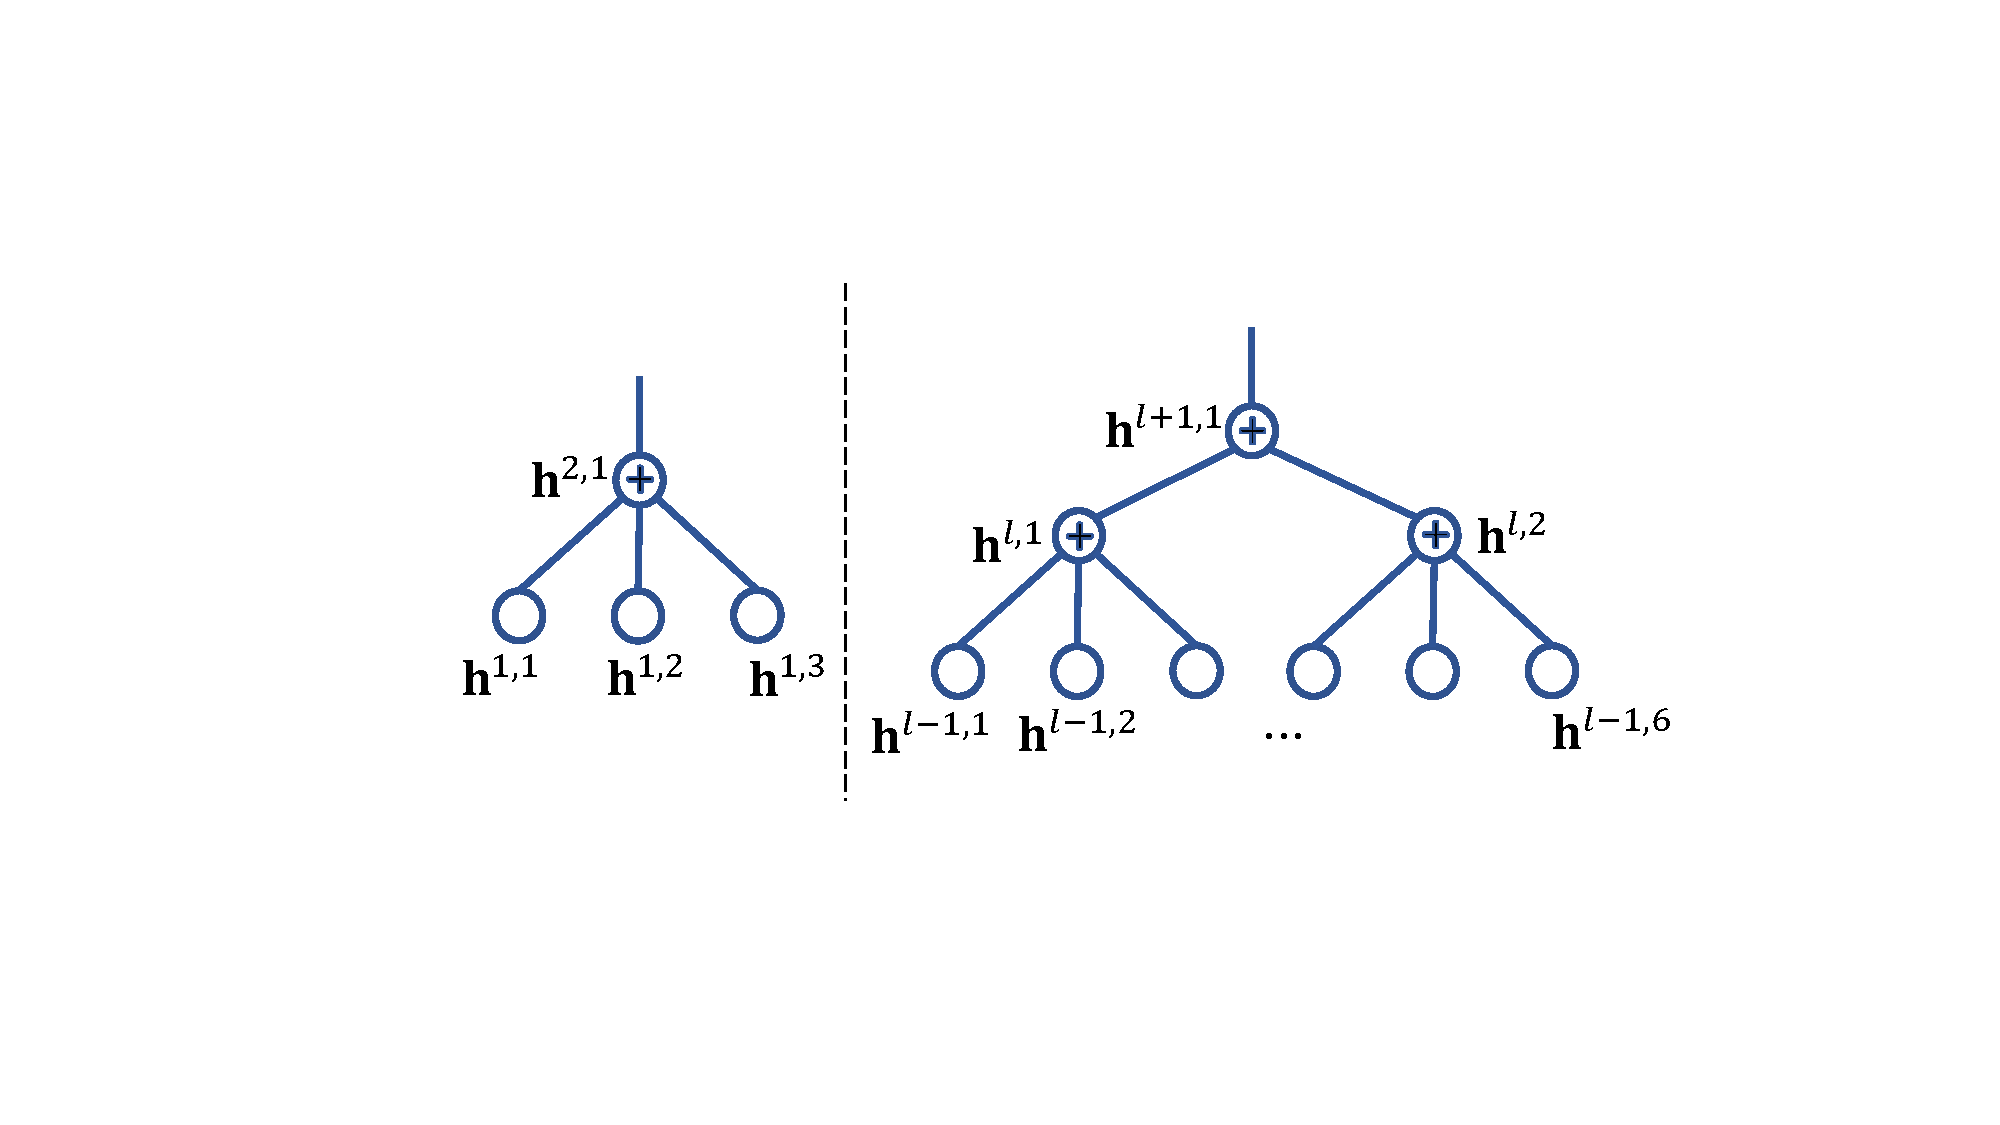
\includegraphics[width=1.0\linewidth]{fig/node.pdf}
\end{center}
\vspace{-0.2in}
\caption{ {\small (Left) The structure of one node. Node $\mathbf{h}^{2,1}$ connects with its children with invertible functions. The messages from its children are aggregated at $\mathbf{h}^{2,1}$.   (Right)An illustration of the latent structure from layer $l-1$ to $l+1$.  $\mathbf{h}^{h, i}$ means the $i$th latent variable  in layer $l$.}}
\label{fig:node_tree}
\vspace{-0.25in}
\end{wrapfigure}
\subsection{The evidence lower bound of Variational Flow Graphical Model}
Figure~\ref{fig:node_tree} illustrates the tree structure induced by varational flow.  The hierarchical generative network has $L$ layers, and $\mathbf{h}^l$ is the latent variable in layer $l$, and $\theta$ is the parameter vector of the model. The hierarchical generative process of the model is given by 
\begin{align*}
p_{\theta_{\mathbf{f}}}(\mathbf{x}) = \sum_{\mathbf{h}^1, ..., \mathbf{h}^L} p_{\theta_{\mathbf{f}}}(\mathbf{h}^L)p_{\theta_{\mathbf{f}}}(\mathbf{h}^{L-1} | \mathbf{h}^{L}) \cdot \cdot  \cdot  p_{\theta_{\mathbf{f}}}(\mathbf{x} | \mathbf{h}^{1}) .
\end{align*}
$p_{\theta_{\mathbf{f}}}(\mathbf{h}^{l-1} | \mathbf{h}^{l})$ is modeled with an invertible normalizing flow function. The hierarchical recognition network is factorized by
\begin{align*}
q_{\theta_{\mathbf{f}}}(\mathbf{h}| \mathbf{x}) =  q_{\theta_{\mathbf{f}}}(\mathbf{h}^1 | \mathbf{x})  q_{\theta_{\mathbf{f}}}(\mathbf{h}^2 | \mathbf{h}^1) \cdot \cdot  \cdot  q_{\theta_{\mathbf{f}}}(\mathbf{h}^{L} | \mathbf{h}^{L-1}),
\end{align*}
where $\mathbf{h}=\{\mathbf{h}^1, \cdots, \mathbf{h}^L \}$ denotes all latent variables. For node $i$, we use $\mathbf{h}^{(i)}$ as the forward evidence message receives from its children, and $\widehat{\mathbf{h}}^{(i)}$ as the  reconstruction of $\mathbf{h}^{(i)}$ with backward message from the rood. $ch(i)$ and $pa(i)$ are node $i$'s child set and parent  set, respectively. Let $\mathbf{f}_{(i, j)}$ be the direct edge~(function) from node $i$  to  $j$, and $\mathbf{f}^{-1}_{ (i, j)}$ or  $\mathbf{f}_{ (j, i)}$  is its inverse function.  We have
\begin{align*}
&  \mathbf{h}^{(j)} = \frac{1}{|ch(j)|} \sum_{i \in ch(j) } \mathbf{f}^{(i,j)}(\mathbf{h}^{(i)}),  \quad \widehat{\mathbf{h}}^{(i)} = \frac{1}{|pa(i)|} \sum_{j \in pa(i) } \mathbf{f}^{-1}_{ (i,j)}(\widehat{\mathbf{h}}^{(j)}) .
\end{align*} 
The inference procedure includes forward and backward message passings, and they corresponds to the encoding and decoding procedures, respectively. The we can compute the layer-wise ELBO for latent states in each layer. With $\mathbf{h}^0 = \mathbf{x}$, the ELBO can be derived as 
\begin{align}  \notag
& \log p(\mathbf{x})  \geqslant \mathcal{L}(\mathbf{x}; \theta) \\
 = & \sum_{l=0}^{L-1}  \mathbb{E}_{q(\mathbf{h}^{l+1}|\mathbf{h}^l)} \bigg[ \log p( \mathbf{h}^{l}|  \widehat{\mathbf{h}}^{l+1})   \bigg] +  \sum_{l=1}^{L-1}   \textbf{\text{H}}(\mathbf{h}^l | \mathbf{h}^{l-1} )   -   \textbf{\text{KL}}\big(q(\mathbf{h}^L | \mathbf{h}^{L-1} )   | p(\mathbf{h}^L)  \big) .  \label{eq:elbo_tree}
\end{align}
The derivation of the ELBO can be found in the Appendix. The first term of ELBO is the reconstruction for each layer: $\mathbf{x}$ and the latent representations $\mathbf{h}^1, ..., \mathbf{h}^{L-1}$. The second and third terms are the regularizations for the latent representation. The nodes are connected with invertible functions such as flow-based models~\cite{Dinh2016DensityEU} to achieve tractable message passing. 

As shown in Figure~\ref{fig:node_tree}-(Left), a node in a flow-graph can has multiple children and multiple parents. Each node has the forward messages from the input data samples and the backward messages from the root.  If all the nodes have only one parent, then the structure is a tree. If there are nodes have multiple parents, the graph will be a DAG~(directed acyclic graph). It is easy to extend the ELBO~\eqref{eq:elbo_tree} to DAGs with topology ordering  of the nodes and thus the layer number. We have the ELBO for a DAG structure as follows
\begin{align}  \notag
 \log p(\mathbf{x}) \geqslant \mathcal{L}(\mathbf{x}; \theta) 
= &  \sum_{i \in \mathcal{G}  \setminus  \mathcal{R}_{ \mathcal{G} }  }  \mathbb{E}_{q(\mathbf{h}^{pa(i)}|\mathbf{h}^{ch(pa(i))})} \bigg[ \log p( \mathbf{h}^{(i)}|  \widehat{\mathbf{h}}^{pa(i)})   \bigg]\\
 & +  \sum_{i \in \mathcal{G}  \setminus  \mathcal{R}_{ \mathcal{G} }  } \textbf{\text{H}}(\mathbf{h}^{(i)} | \mathbf{h}^{ch(i)} )   -    \sum_{i \in  \mathcal{R}_{ \mathcal{G} }  }  \textbf{\text{KL}}\big(q(\mathbf{h}^{(i)} | \mathbf{h}^{ch(i)} )   | p(\mathbf{h}^{(i)})  \big) . \label{eq:elbo_dag}
 \end{align}
Here $\mathcal{G}$ stands for the node set of the GAG, and $\mathcal{R}_{ \mathcal{G}}$ is the set of root or source nodes. 
 Assume there are $k$ leaf nodes on a tree or a DAG model, and they correspond to $k$ sections of the input sample $\mathbf{x} = [\mathbf{x}^{(1)}, ..., \mathbf{x}^{(k)}]$.   The terms in both~\eqref{eq:elbo_tree} and~\eqref{eq:elbo_dag} are computed with . We provide more details about the nodes in next subsection.
 
\begin{figure*}[!htbp] %{r{0.4\textwidth}
\begin{center}
 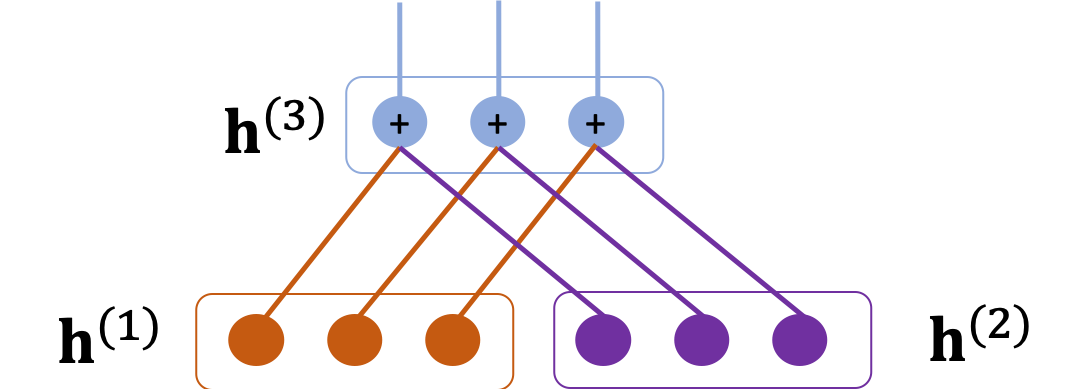
\includegraphics[width=0.43\linewidth]{fig/node_aggre_sum.png}
 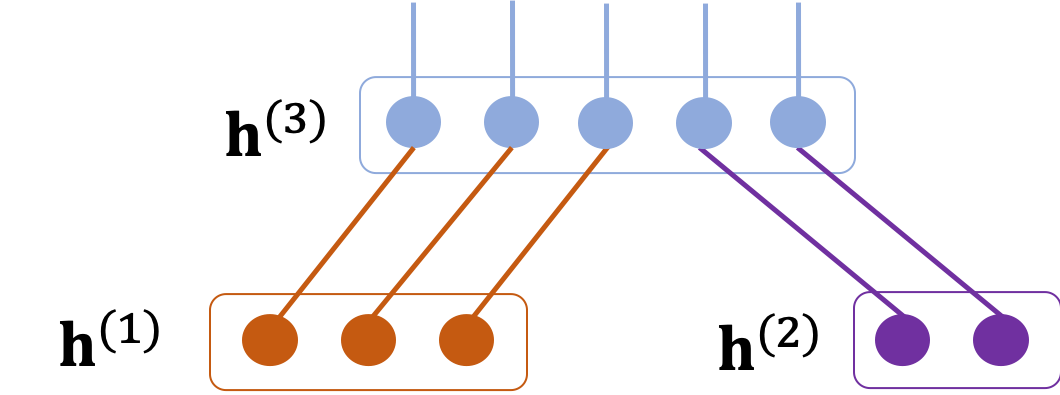
\includegraphics[width=0.43\linewidth]{fig/node_aggre_cat.png}
\end{center}
   \caption{(Left) Aggregation with average. (Right) Aggregation with concatenation. }
\label{fig:node_aggre}
\end{figure*}

\subsection{Node Aggregation}

We use normal distribution as the prior for all the nodes. There are two approaches to aggregate signals from different nodes:  average based and concatenation based  aggregation. They are illustrated by the left and right plots of Figure~\ref{fig:node_aggre}, respectively. Concatenation based aggregation is simple and straight forward. We will focus on average aggregation nodes. We assume each entry of a hidden node follow normal distribution, i.e., $\mathbf{h}_j^{(i)} \sim \mathbb{N}(\mu_j^{(i)}, \sigma^2)$ for node $i$'s $j$th entry. We use the same $\sigma$ value across all nodes. Let's assume a model  only has one average aggregation node as shown in Figure~\ref{fig:node_aggre}-left. According to with the ELBO 
\begin{align} \notag
\log p(\mathbf{x})  \geqslant \mathcal{L}(\mathbf{x}; \theta_{\mathbf{f}})
=&\mathbb{E}_{q(\mathbf{h}^1 | \mathbf{x})} \big[\log p(\mathbf{x}|\widehat{\mathbf{h}}^1)\big] + \mathbf{H}(\mathbf{h}^1 | \mathbf{x}) + \\ \label{eq:average}
&\mathbb{E}_{q(\mathbf{h}^2 | \mathbf{h}^1)} \big[\log p(\mathbf{h}^1|\widehat{\mathbf{h}}^2)\big] - \textbf{\text{KL}}\big(q(\mathbf{h}^2 | \mathbf{h}^1) | p(\mathbf{h}^2)\big).
\end{align} 
In an average aggregation node $i$, the parent value is the mean of its children, i.e., $\mathbf{h}^{(i)} = \frac{1}{|ch(i)|} \sum_{j \in ch(i)} \mathbf{h}^{(j)}$. The  children  share the same reconstruction value with its parent, i.e., $\widehat{\mathbf{h}}^{(j)} = \widehat{\mathbf{h}}^{(i)}, \forall j \in ch(i)$. In an one aggregation node model with $\mathbf{h}^{(r)}$ as the root, we have  $\widehat{\mathbf{h}}^{(r)} = \mathbf{h}^{(r)} = \frac{1}{k}\sum_{t=1}^k \mathbf{h}^{(t)} $, and $ \widehat{\mathbf{h}}^{(1)} = ... = \widehat{\mathbf{h}}^{(k)}= \widehat{\mathbf{h}}^{(r)}$. Here $k$ is the children number, and $k=3$ in Figure~\ref{fig:node_aggre}-left. Given one data sample $\mathbf{x}$, the reconstruction terms in ELBO~\eqref{eq:average} are computed with 
\begin{align}\notag
\log p(\mathbf{x}|\widehat{\mathbf{h}}^1) + \log p(\mathbf{h}^1|\widehat{\mathbf{h}}^2)
=&-\sum_{t=1}^k\bigg\{ \frac{1}{2\sigma^2_{\mathbf{x}}}\big|\big| \mathbf{x}^{(t)} - \mathbf{f}_t^{-1}(\widehat{\mathbf{h}}^{(t)})\big|\big|^2 +  \frac{1}{2\sigma^2}\big|\big| \mathbf{h}^{(t)} -\widehat{\mathbf{h}}^2 \big|\big|^2 \bigg\} +C \\
=&-\sum_{t=1}^k\bigg\{ \frac{1}{2\sigma^2_{\mathbf{x}}}\big|\big| \mathbf{x}^{(t)} - \mathbf{f}_t^{-1}(\widehat{\mathbf{h}}^{(r)})\big|\big|^2 +  \frac{1}{2\sigma^2}\big|\big|  \mathbf{f}_t(\mathbf{x}^{(t)}) - \widehat{\mathbf{h}}^{(r)}\big|\big|^2 \bigg\} +C \label{eq:yllk} .
\end{align} 
Here $C=-dk\ln(2\pi)-\frac{dk}{2}\ln(\sigma_{\mathbf{y}}^2)-\frac{dk}{2}\ln(\sigma^2)$, and $\mathbf{f}_t$ connects $\mathbf{h}^{(t)}$ and $\mathbf{x}^{(t)}$. We use constant values for both  $\sigma^2_{\mathbf{y}}$ and $\sigma^2$, hence the value of $C$ is constant as well. We use the latent variables from a batch of training samples to approximate the entry \textbf{H} and \textbf{KL} terms in~\eqref{eq:average}. We take the parent and children involved an aggregation operation as one node in the graphical figures, e.g., Figure~\ref{fig:node_tree}. 

\subsection{Inference on Sub-graphs }
Given a trained VFG model, we can infer a node's state given observed nodes. Relations between variables at different nodes  can also be infered with the model. The prediction of leaf node $i$ dependents on its parents, i.e.,
\begin{wrapfigure}{r}{.5\textwidth}
\begin{center}
 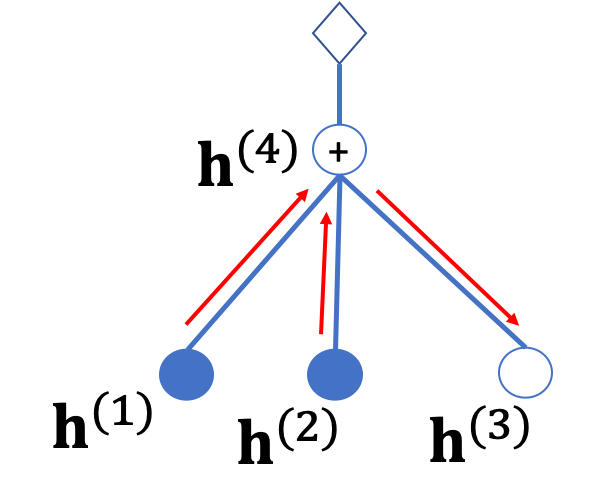
\includegraphics[width=0.4\linewidth]{fig/two_layer_infer.png}
 \hspace{0.15in}
 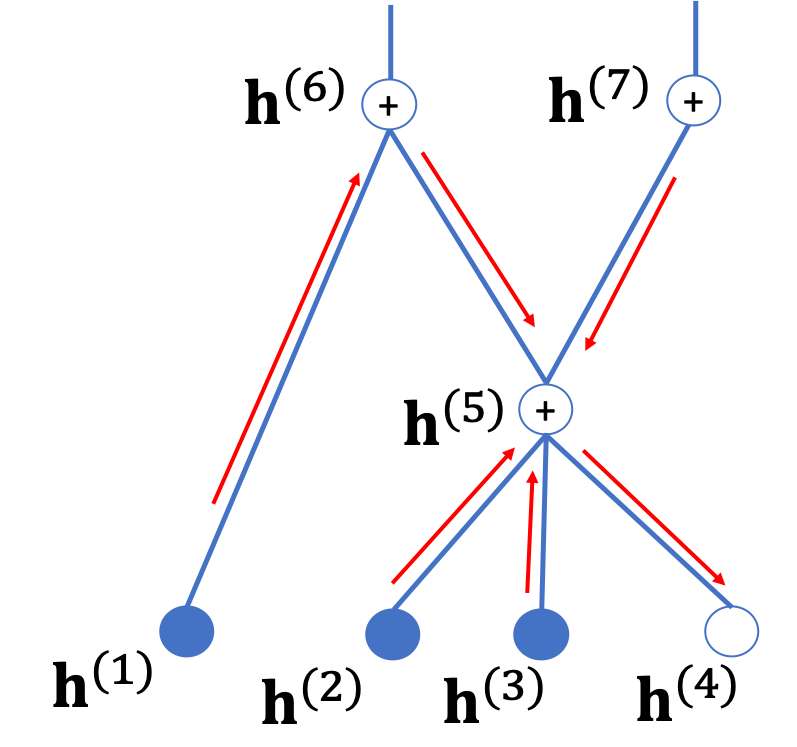
\includegraphics[width=0.5\linewidth]{fig/dag_infer.png}
\end{center}
\vspace{-0.2in}
 \caption{{\small (Left) Inference of single aggregation node model. Node 4 aggregates messages from node 1 and 2, and then pass  the updated state to node 3 for prediction. (Right) Inference on a DAG model. Observed node states are gathered in node 5 to predict the state of node 4.}}
\label{fig:two_layer_infer}
\vspace{-0.23in}
\end{wrapfigure}
\begin{align*}
p(\mathbf{h}^{(i)} | \mathbf{h}^{pa(i)}) & = p(\mathbf{h}^{pa(i)}) \bigg|\det(\frac{\partial \mathbf{h}^{pa(i)} }{\partial \mathbf{h}^{(i)}})\bigg|  =
p(\mathbf{h}^{pa(i)}) \big|\det(\mathbf{J}_{pa(i)}(i))\big| .
\end{align*} 
The hidden state of the parent node $s$ in a single aggregation model can be approximated by the observed children,
$\mathbf{h}^{(s)}  = \frac{1}{|ch(s)|}\sum_{i \in ch(s) \cap O} \mathbf{h}^{(i)} .$
%\begin{figure}[!htbp] %{r{0.4\textwidth}
Here $O$ is the set of observed leaf nodes. Figure~\ref{fig:two_layer_infer}-left illustrates one example of this case. 
For a node in a tree or DAG model, its state is updated with messages from its children with updating and then pass it to  children without updating. Figure~\ref{fig:two_layer_infer}-right illustrates  inference on a DAG. The tree and DAG structures enable the model to perform message passing  among the nodes.  We have the following lemma regarding the relation between two leaf nodes. 
\begin{lemma}\label{lm:apprx}
Let $\mathcal{G}$ be a well trained tree structured variational flow graphical model with $L$ layers, and $i$ and $j$ are two leaf nodes with $a$ as the closest common ancestor. Given observed value at node $i$, the value of node $j$ can be approximated with   $\widehat{\mathbf{x}}^{j} \approx  \mathbf{f}_{(a,j)}(\mathbf{f}_{(i, a)}(\mathbf{x}^{(i)}))$. Here $\mathbf{f}_{(i, a)}$ is the flow function path from node $i$ to node $a$. The conditional density of $\mathbf{x}^{(j)}$ given $\mathbf{x}^{(i)}$ can be approximated with 
\begin{align} \label{eq:cond_llk}
\log p(\mathbf{x}^{(j)} | \mathbf{x}^{(i)}) &\approx  \log p(\widehat{\mathbf{h}}^L) -  \frac{1}{2} \log \big(\det \big(\mathbf{J}_{\widehat{\mathbf{x}}^{(j)}}(\widehat{\mathbf{h}}^L)^\top\mathbf{J}_{\widehat{\mathbf{x}}^{(j)}}(\widehat{\mathbf{h}}^L)\big) \big).
\end{align}
\end{lemma}

\begin{remark}\label{rmk:apprx_mul}
Let $O$ be the set of observed leaf nodes, $j$ be an unobserved node, and $a$ is the closest ancestor of $O$ and $a$. Then the state of $j$ can be imputed with  $\widehat{\mathbf{x}}^{j} \approx  \mathbf{f}_{(a,j)}(\mathbf{f}_{(O, a)}(\mathbf{x}^{(i)}))$.  $\mathbf{f}_{(O, a)}$ is the flow function path from all nodes in $O$ to $a$, and approximation~\eqref{eq:cond_llk} still holds for $p(\mathbf{x}^{(j)} | \mathbf{x}^{O})$.
\end{remark}

These results can be easily extended to DAG models. The proof of Lemma~\ref{lm:apprx} can be found in the appendix. 

\subsection{Algorithm and Implementation}
Model parameters $\theta_{\mathbf{f}}$ are learned by maximizing the ELBO~\eqref{eq:elbo_tree} or~\eqref{eq:elbo_dag}.  The latent variables are computed in forward message passing and their reconstructions are computed in backward message passing.  We use the empirical variance in a batch of training samples to approximate the entropy and \textbf{KL} terms. Ignoring  explicit variance  for all latent nodes enable us to use flow-based models as the encoders as well as the decoders. 

\begin{algorithm}[h!]
   \caption{Inference model parameters with  forward and backward message propagation}
   \label{alg:main}
\begin{algorithmic}
   \STATE {\bfseries Input:} Data distribution $\mathcal{D}$,  $\mathcal{G} = \{\mathcal{V}, \mathbf{f}\}$
   \REPEAT
   \STATE Sample minibatch $b$ samples $\{\mathbf{x}_1, ..., \mathbf{x}_b \}$ from $\mathcal{D}$;
   \FOR{$i \in \mathcal{V}$}
   \STATE $\mathbf{h}^{(i)} = \frac{1}{|ch(i)|} \sum_{j \in ch(i) } \mathbf{f}_{(j,i)}(\mathbf{h}^{(j)})$;  \textcolor{blue}{// forward message passing}
   \ENDFOR
    \STATE  $\mathbf{h} =  \{\mathbf{h}^{(1)}, ...,  \mathbf{h}^{(|\mathcal{V}|)}  \}$;
    \FOR{$i \in \mathcal{V}$}
   \STATE $\widehat{\mathbf{h}}^{(i)} = \frac{1}{|pa(i)|} \sum_{j \in pa(i) } \mathbf{f}^{-1, (i,j)}(\widehat{\mathbf{h}}^{(j)}) $;  \textcolor{blue}{// backward message passing}
   \ENDFOR
    \STATE  $ \widehat{\mathbf{h}} =  \{\widehat{\mathbf{h}}^{1}, ...,  \widehat{\mathbf{h}}^{(|\mathcal{V}|)}  \}$;
    
    \STATE Updating flow-graph $\mathcal{G}$ by descending the gradient $\bigtriangledown_{\theta_{\mathbf{f}}}\frac{1}{b} \sum_{i=1}^b  \big[ -\mathcal{L}(\mathbf{x}_b; \theta_{\mathbf{f}} ) \big] $ ;
   %\ENDFOR 
   \UNTIL{Converge}
\end{algorithmic}
\end{algorithm}




\section{Theory}
The proposed VFG model 

\section{Experiments}


\subsection{Imputation}

\subsubsection{Baselines}
The data set is divided into training and testing sets. The model is trained with the training set, then it is used to infer the missing entries of samples in the testing set. We use the following baselines for data imputation.

\begin{itemize}
\item \textbf{Mean Value} \ We can directly use the mean values in the corresponding position of training set to replace the missing entries in the testing set.  

\item \textbf{Iterative Imputation} A strategy for imputing missing values by modeling each feature with missing values as a function of other features in a Round-Robin fashion. We choose the KNeighborRegressor as the specific function~\cite{scikit-learn}.

\item \textbf{KNN} \  To use K-Nearest Neighbor for data imputation,  we compare the non-missing entries of each sample to the training set and use the  average of top $k$ samples to impute the missing entries. 

\item \textbf{Multivariate Imputation by Chained Equation (MICE)} \ This method impute the missing entries with multiple  rounds of inference. The method can handle different kind data types.
\end{itemize}

\subsubsection{Evaluation with Synthetic Data  }
In this set of experiments, we study the proposed model with synthetic data sets.
We use two latent variables, i.e. Z

We generate 1000 data points for model training, and each data sample  has 8 dimension with 2 latent variables.  The relation between the latent variables and the 

Figure~\ref{fig:elbo} gives the ELBO values of the proposed method. 

\begin{figure}[!htbp]
    \centering
    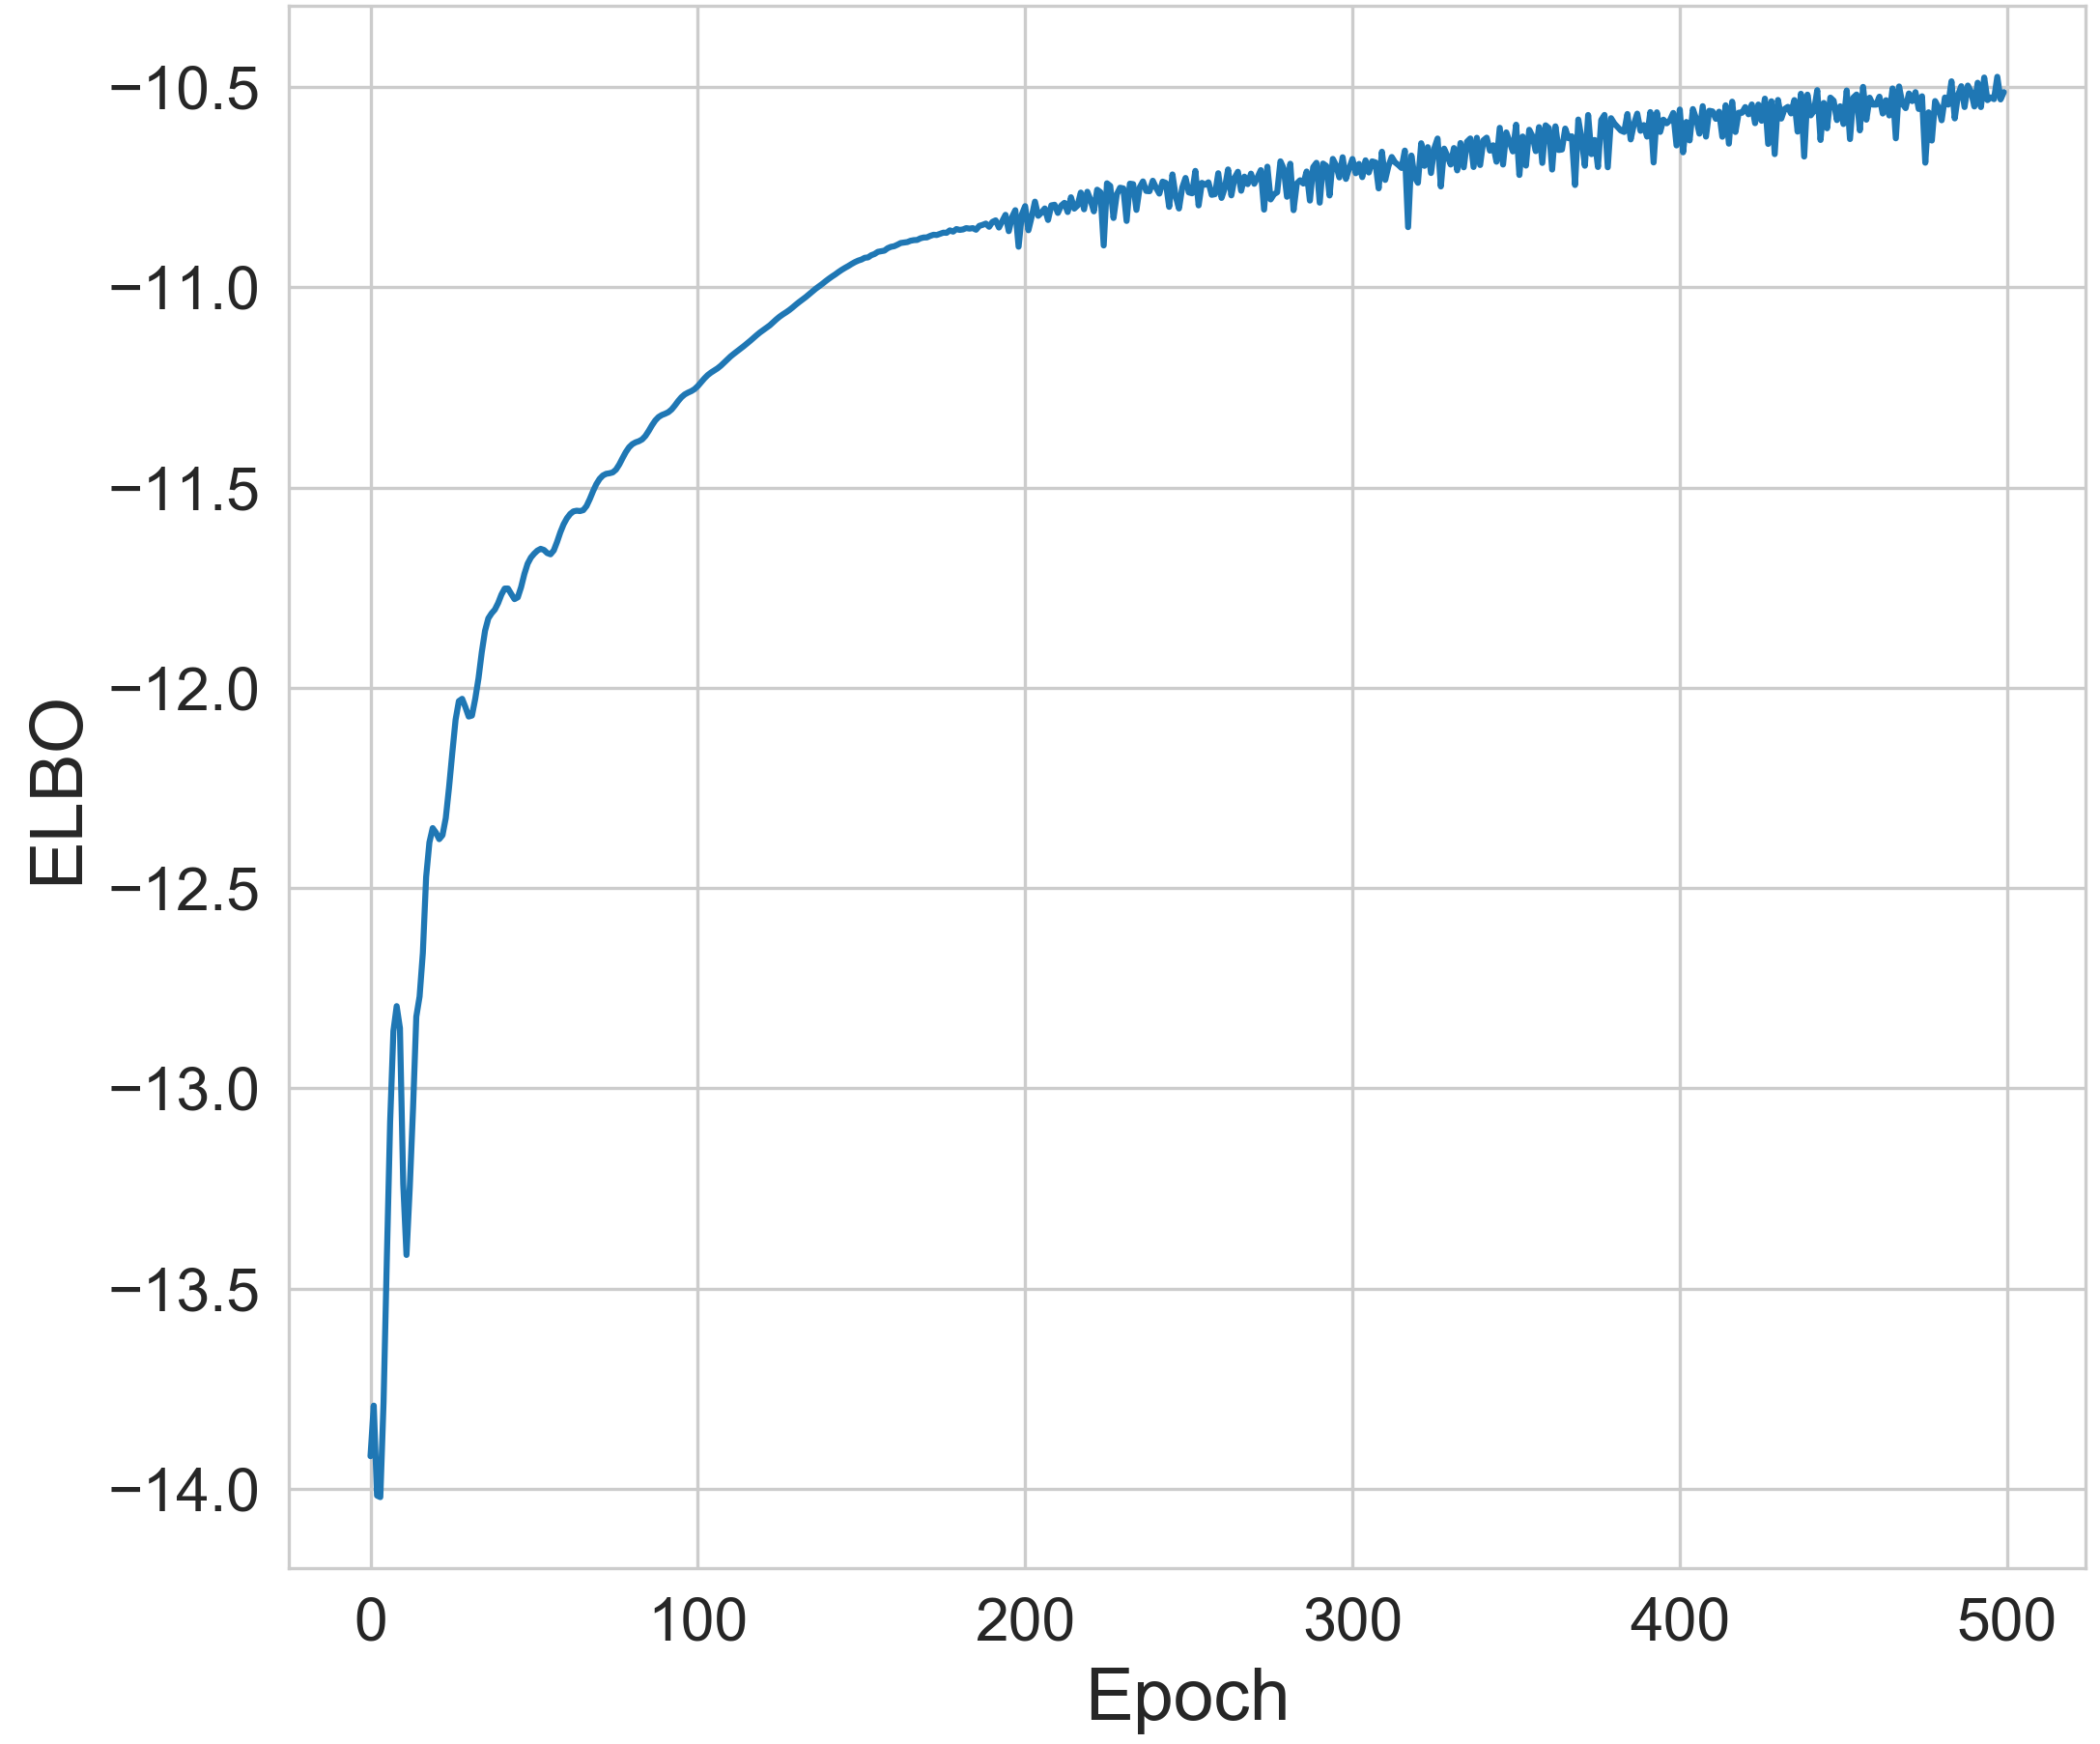
\includegraphics[width=2.3in]{fig/elbo.png}
    \caption{ELBO on the synthetic data}
    \label{fig:elbo}
\end{figure}

\begin{figure*}[!htbp]
    \centering
    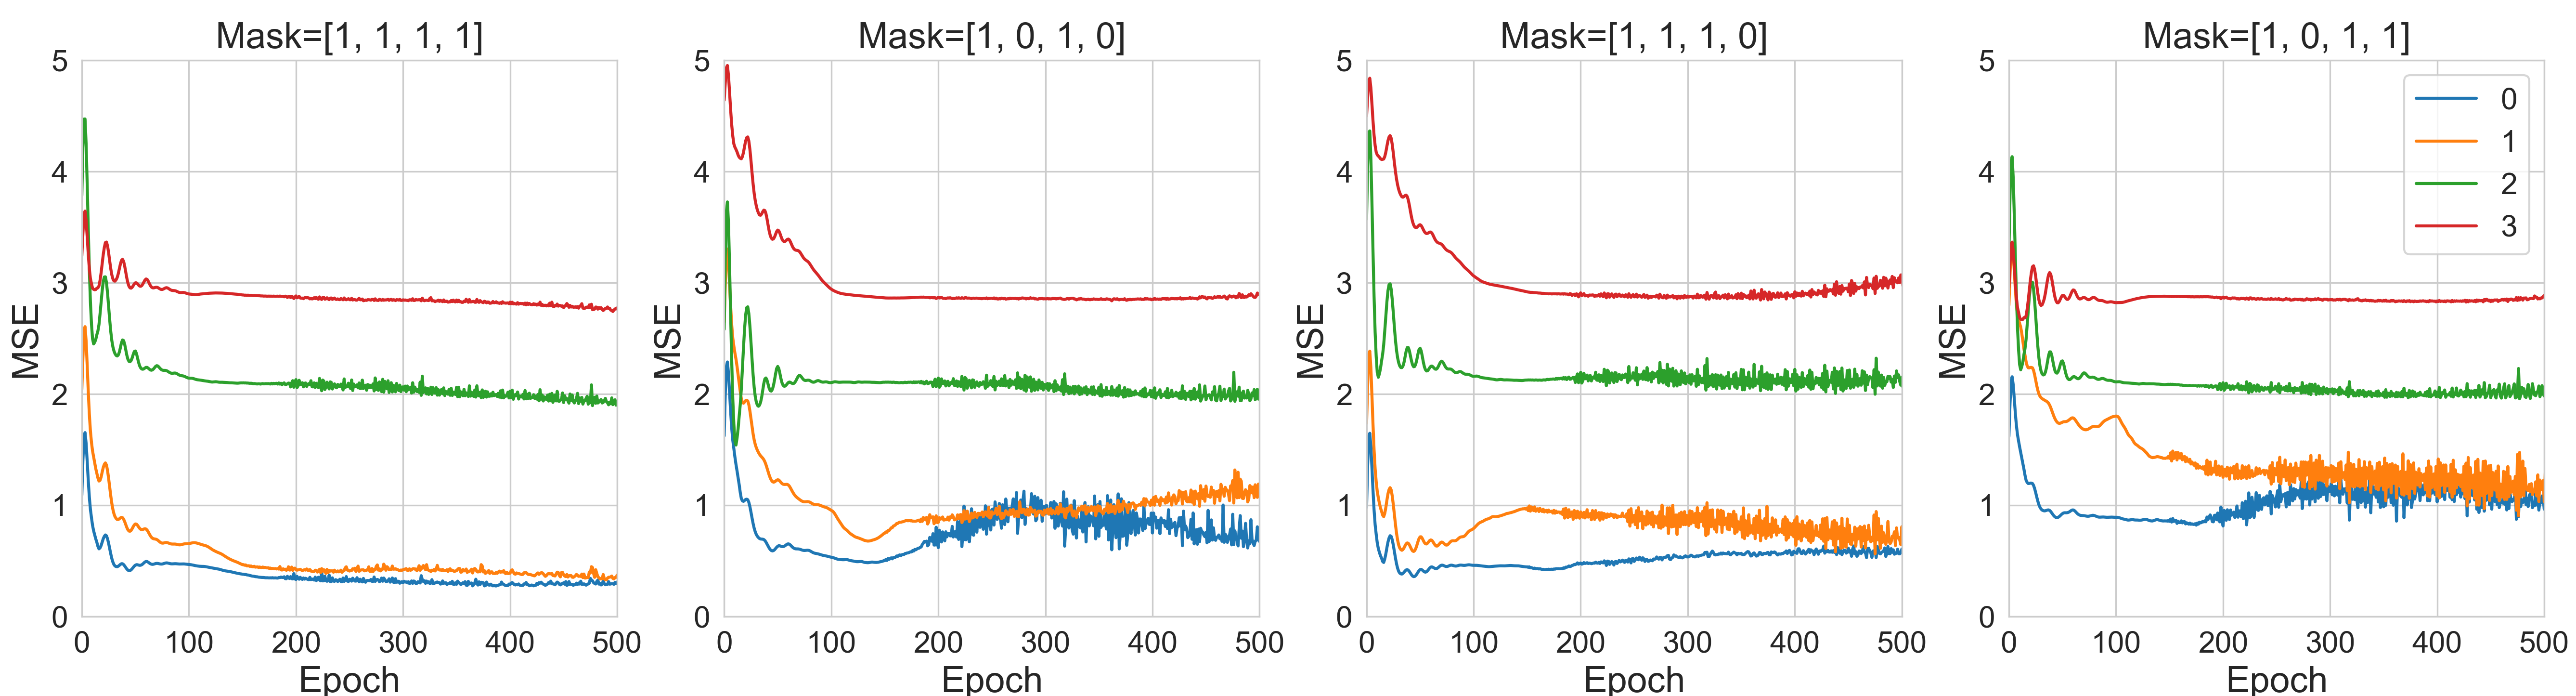
\includegraphics[width=0.95\textwidth]{fig/mse.png}
    \caption{Imputation with $\mathsf{Mask}$ on the child nodes [0, 1, 2, 3] indicated by colored legends. }
    \label{fig:mse}
\end{figure*}

%\subsubsection{Data Imputation}

%\subsubsection{Graph Structure Recovery}
\begin{table}[t!]
\begin{center}
%\vspace{0.15in}
\caption{Imputation Results on Synthetic Data.} \label{tab:causality2}
\begin{tabular}{l | c  }\hline
Methods & Imputation MSE  \\
\hline
Mean Value &8.43 \\
\hline
MICE &8.38 \\
\hline
Iterative Imputation & 2.64 \\
\hline
KNN (k=3) &0.14 \\
\hline
KNN (k=5) &0.18 \\
\hline
Proposed &  1.45  \\  
\hline
\end{tabular}
\end{center}
\end{table}

\subsubsection{Arrhythmia Data Set}
We further investigate the method on a tabular data set.  The Arrhythmia~\cite{Dua:2019}  data set is  obtained from the ODDS repository. The smallest classes, including 3, 4, 5, 7, 8, 9, 14, and 15, are combined to form the anomaly class, and the rest of the classes are combined to form the normal class. Table 4 shows the anomaly detection results with different methods. 


\subsection{Disentanglement on MNIST}


\section{Conclusion}
% \section*{Acknowledgment}

% The preferred spelling of the word ``acknowledgment'' in America is without 
% an ``e'' after the ``g''. Avoid the stilted expression ``one of us (R. B. 
% G.) thanks $\ldots$''. Instead, try ``R. B. G. thanks$\ldots$''. Put sponsor 
% acknowledgments in the unnumbered footnote on the first page.

\bibliographystyle{iclr2021_conference}
\bibliography{iclr2021_conference}

\clearpage
\section*{Appendix A.  ELBO of Tree Models}\label{appd:tree_elbo}

The hierarchy generative network as given in Figure~\ref{fig:tree-d}. For each pair of connected nodes, the edge is linked with an invertible function. We use $\theta$ to represent the parameters for all the edges.
The forward message passing starts from $\mathbf{x}$ and ends at $\mathbf{h}^L$, and backward message passing is in the reverse direction. 
 Then the
 likelihood for the data is given by
\begin{align*}
p(\mathbf{x}| \mathbf{\theta}) = \sum_{\mathbf{h}^1, ..., \mathbf{h}^L} p(\mathbf{h}^L | \theta)p(\mathbf{h}^{L-1} | \mathbf{h}^{L},\theta) \cdot \cdot  \cdot  p(\mathbf{x} | \mathbf{h}^{1}, \theta) .
\end{align*}

\begin{figure}[!htbp]
    \centering
    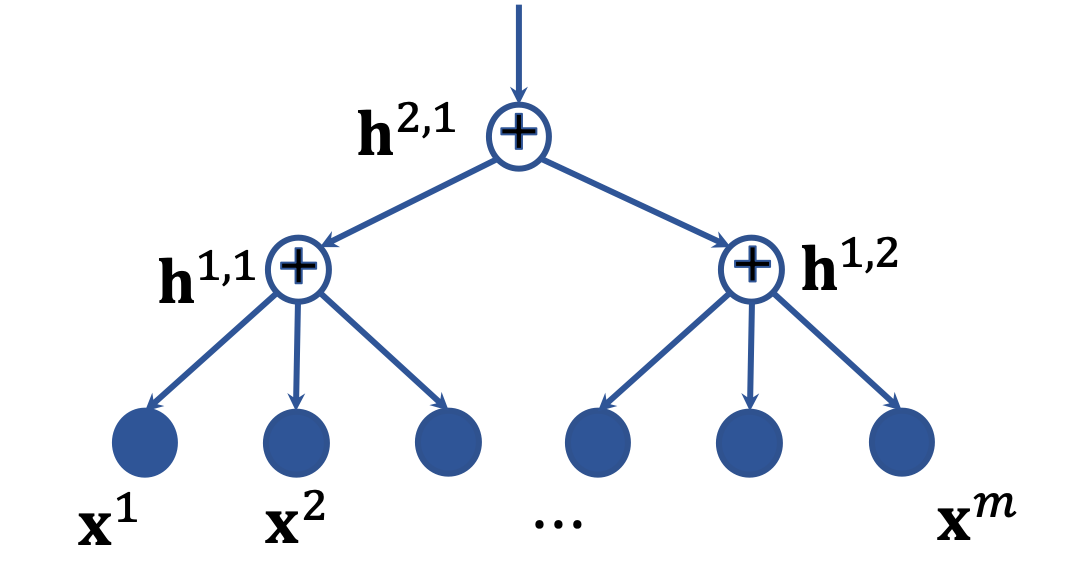
\includegraphics[width=2.3in]{fig/tree_direct.png}
    \caption{Tree structure.}
    \label{fig:tree-d}
\end{figure}

With the flow-based ensemble model, each edge is invertible.   The hierarchy of recognition network is the procedure from top to down of the structure as shown in Figure~\ref{fig:tree-d}.  Similarly, with the Markov property of the structure, the posterior density of the latent 
variables is given by
\begin{align*}
q(\mathbf{h}| \mathbf{x}, \theta ) = q(\mathbf{h}^1 | \mathbf{x}, \theta)  q(\mathbf{h}^2 | \mathbf{h}^1, \theta) \cdot \cdot  \cdot  q(\mathbf{h}^{L} | \mathbf{h}^{L-1}, \theta) .
\end{align*}
It can be simplified as 
\begin{align*}
q(\mathbf{h}| \mathbf{x}) = q(\mathbf{h}^1 | \mathbf{x})  q(\mathbf{h}^2 | \mathbf{h}^1) \cdot \cdot  \cdot  q(\mathbf{h}^{L} | \mathbf{h}^{L-1}) .
\end{align*}
We also have 
\begin{align} \label{eq:chain}
q(\mathbf{h}| \mathbf{x}) = q(\mathbf{h}^1 | \mathbf{x})  q(\mathbf{h}^{2:L} | \mathbf{h}^1) .
\end{align}

To derive the ELBO of a hierarchy model, we take all  layers of latent variables as the latent vector in conventional VAE, and we have 
\begin{align*}
&\log p(\mathbf{x})\\
=&  \mathbb{E}_{q(\mathbf{h} | \mathbf{x})} \bigg[ \log  \frac{p(\mathbf{x}, \mathbf{h})}{p(\mathbf{h}|\mathbf{x})} \bigg] \\
=&  \mathbb{E}_{q(\mathbf{h} | \mathbf{x})} \bigg[ \log  \frac{p(\mathbf{x}, \mathbf{h})}{q(\mathbf{h}|\mathbf{x})}   \frac{q(\mathbf{x}, \mathbf{h})}{p(\mathbf{h}|\mathbf{x})} \bigg] \\
=&  \underbrace{\mathbb{E}_{q(\mathbf{h} | \mathbf{x})} \bigg[ \log  \frac{p(\mathbf{x}, \mathbf{h})}{q(\mathbf{h}|\mathbf{x})}  \bigg]}_{\underset{\text{(ELBO)}}{\mathcal{L}_{\theta}(x)}} +   \underbrace{\mathbb{E}_{q(\mathbf{h} | \mathbf{x})} \bigg[ \log \frac{q(\mathbf{h} |\mathbf{x})}{p(\mathbf{h}|\mathbf{x})} \bigg]}_{\text{KL}\big(q(\mathbf{h} |\mathbf{x}) | p(\mathbf{h}|\mathbf{x})\big)} .
\end{align*}
With $\text{KL}\big(q(\mathbf{h} |\mathbf{x}) | p(\mathbf{h}|\mathbf{x})\big) \geq 0$, we have 

\begin{align}  \label{eq:tree_elbo}
&\log p(\mathbf{x})  \geq  \mathcal{L}_{\theta}(x) \\  \notag
=&  \mathbb{E}_{q(\mathbf{h} | \mathbf{x})} \bigg[ \log  \frac{p(\mathbf{x}, \mathbf{h})}{q(\mathbf{h}|\mathbf{x})}  \bigg]  \\  \notag
=&  \mathbb{E}_{q(\mathbf{h}^{1:L} | \mathbf{x})} \bigg[ \log  \frac{p(\mathbf{x} | \mathbf{h}^{1:L}) p( \mathbf{h}^{1:L})}{q(\mathbf{h}^{1:L}|\mathbf{x})}  \bigg]  \\   \notag
 =&  \mathbb{E}_{q(\mathbf{h}^{1:L} | \mathbf{x})} \bigg[  \log p(\mathbf{x} | \mathbf{h}^{1:L})  \bigg]  +  \mathbb{E}_{q(\mathbf{h}^{1:L} | \mathbf{x})} \bigg[ \log   \frac{p( \mathbf{h}^{1:L})}{q(\mathbf{h}^{1:L}|\mathbf{x})}  \bigg]   \\    \label{eq:layer0_a}
=&  \mathbb{E}_{q(\mathbf{h}^{1:L} | \mathbf{x})} \bigg[ \log p(\mathbf{x} | \mathbf{h}^{1})  \bigg]  +  \mathbb{E}_{q(\mathbf{h}^{1:L} | \mathbf{x})} \bigg[ \log     \frac{p( \mathbf{h}^{1:L})}{q(\mathbf{h}^{1:L}|\mathbf{x})}  \bigg]  \\ 
=&  \underbrace{ \mathbb{E}_{q(\mathbf{h}^{1} | \mathbf{x})} \bigg[ \log  p(\mathbf{x} | \mathbf{h}^{1})  \bigg] }_{  \parbox{10.5em}{Reconstruction of the data given hidden layer 1}}  +  \underbrace{  \mathbb{E}_{q(\mathbf{h}^{1:L} | \mathbf{x})} \bigg[ \log  \frac{p( \mathbf{h}^{1:L})}{q(\mathbf{h}^{1:L}|\mathbf{x})}  \bigg] }_{-\text{KL}^{1:L}}.     \label{eq:layer0_b}
\end{align}

The first term in~\eqref{eq:layer0_a} is due to $p(\mathbf{x}|\mathbf{h}^{1:L}) =  p(\mathbf{x}|\mathbf{h}^{1})$. The first term in~\eqref{eq:layer0_b} is due to that the expectation is regarding $\mathbf{h}^{1}$. The hidden variables $\mathbf{h}^{l+1:L}$ can be taken as the parameters for $\mathbf{h}^l$'s  prior distribution .  We expand the minus KL term in~\eqref{eq:layer0_b} as follows
\begin{align} \label{eq:kl_1}
&-\text{KL}^{1:L} \\ \notag
=& \mathbb{E}_{q(\mathbf{h}^{1:L} | \mathbf{x})} \bigg[ \log  \frac{p( \mathbf{h}^{1:L})}{q(\mathbf{h}^{1:L}|\mathbf{x})}  \bigg]   \\ \notag
= &   \mathbb{E}_{q(\mathbf{h}^{1:L} | \mathbf{x})} \bigg[ \log  \frac{p( \mathbf{h}^{1}|  \mathbf{h}^{2:L}) p( \mathbf{h}^{2:L})  }{\underbrace{ q(\mathbf{h}^{1}|\mathbf{x}) q(\mathbf{h}^{2:L}|\mathbf{h}^1)}_{\text{Due to}~\eqref{eq:chain}} }  \bigg] \\ \notag
=&  \underbrace{  \mathbb{E}_{q(\mathbf{h}^{1:L} | \mathbf{x})} \bigg[ \log  \frac{p( \mathbf{h}^{1}|  \mathbf{h}^{2:L}) p( \mathbf{h}^{2:L})  }{ q(\mathbf{h}^{2:L}|\mathbf{h}^1)}  \bigg]  }_{(a)} +   \underbrace{\mathbb{E}_{q(\mathbf{h}^{1:L} | \mathbf{x})} \bigg[ \log \frac{1}{q(\mathbf{h}^{1}|\mathbf{x}) } \bigg] }_{(b)}  \notag
\end{align}

Given a batch of data, we take the inference in each layer as encoding and decoding procedures. In forward message passing, the hidden layer $\mathbf{h}^l$  only depends on its previous layer $l-1$. 
The logarithm term in (a) only relates to hidden states $\mathbf{h}^{1:L}$.  With the feed message from the child layer $\overrightarrow{\mathbf{h}}^{(i)}$ and the reconstruct message $\overleftarrow{\mathbf{h}}^{(i)}$  from the parent layer, we can derive the ELBO term for the likelihood of  $\overrightarrow{\mathbf{h}}^{(i)}$ .  With~\eqref{eq:chain}, given the hidden states $\mathbf{h}^1$ samples from layer 0, we have 
\begin{align} \label{eq:kl_a}
(a)  &=   \mathbb{E}_{q(\mathbf{h}^{1}|\mathbf{x})} \bigg[  \mathbb{E}_{q(\mathbf{h}^{2:L}|\mathbf{h}^1)} \bigg[ \log  \frac{p( \mathbf{h}^{1}|  \mathbf{h}^{2:L}) p( \mathbf{h}^{2:L})  }{ q(\mathbf{h}^{2:L}|\mathbf{h}^1)}  \bigg]    \bigg] .
\end{align}
The inner expectation is actually the ELBO for layer hidden variable $\mathbf{h}^1$. Hence
\begin{align} \notag
 &\mathbb{E}_{q(\mathbf{h}^{2:L}|\mathbf{h}^1)} \bigg[ \log  \frac{p( \mathbf{h}^{1}|  \mathbf{h}^{2:L}) p( \mathbf{h}^{2:L})  }{ q(\mathbf{h}^{2:L}|\mathbf{h}^1)}  \bigg]   \\ \notag
 =&\mathbb{E}_{q(\mathbf{h}^{2:L}|\mathbf{h}^1)} \big[  p( \mathbf{h}^{1}|  \mathbf{h}^{2:L})    \big] + \mathbb{E}_{q(\mathbf{h}^{2:L}|\mathbf{h}^1)} \bigg[ \log  \frac{ p( \mathbf{h}^{2:L})   }{ q(\mathbf{h}^{2:L}|\mathbf{h}^1)}  \bigg]  \\  \label{eq:a_inner}
 =&  \mathbb{E}_{q(\mathbf{h}^{2}|\mathbf{h}^1)} \big[  p( \mathbf{h}^{1}|  \mathbf{h}^{2})    \big] + \mathbb{E}_{q(\mathbf{h}^{2:L}|\mathbf{h}^1)} \bigg[ \log  \frac{ p( \mathbf{h}^{2:L})   }{ q(\mathbf{h}^{2:L}|\mathbf{h}^1)}  \bigg] \\ \notag
  =&  \mathbb{E}_{q(\mathbf{h}^{2}|\mathbf{h}^1)} \big[  p( \mathbf{h}^{1}|  \mathbf{h}^{2})    \big] - \text{KL}^{2:L} .
\end{align}

For the term (b),
\begin{align} \notag
 (b) & = \mathbb{E}_{q(\mathbf{h}^{1:L} | \mathbf{x})} \bigg[ \log \frac{1}{q(\mathbf{h}^{1}|\mathbf{x}) } \bigg] \\ \notag
&=  \mathbb{E}_{q(\mathbf{h}^{1} | \mathbf{x})} \bigg[ \log \frac{1}{q(\mathbf{h}^{1}|\mathbf{x}) } \bigg] \\ \label{eq:kl_b}
& = \text{H}(\mathbf{h}^{1}|\mathbf{x}) .
\end{align}

With~\eqref{eq:kl_1}~\eqref{eq:kl_a}~\eqref{eq:a_inner}~\eqref{eq:kl_b}, 
\begin{align*}
&-\text{KL}^{1:L} =    \mathbb{E}_{q(\mathbf{h}^{1}|\mathbf{x})} \bigg[  \mathbb{E}_{q(\mathbf{h}^{2}|\mathbf{h}^1)} \big[  p( \mathbf{h}^{1}|  \mathbf{h}^{2})    \big]  - \text{KL}^{2:L}  \bigg] +  \text{H}_q(\mathbf{h}^{1}|\mathbf{x}).
\end{align*}

Similarly, for layer $l$, we  have 
\begin{align*} % \label{eq:KL_l}
-\text{KL}^{l:L} 
=  & \mathbb{E}_{q(\mathbf{h}^{l}|\mathbf{h}^{l-1})} \bigg[  \mathbb{E}_{q(\mathbf{h}^{l+1}|\mathbf{h}^l)} \big[  p( \mathbf{h}^{l}|  \mathbf{h}^{l+1})    \big]  - \text{KL}^{l+1:L}  \bigg]   +  \text{H}_q(\mathbf{h}^{l}|\mathbf{h}^{l-1}) \\ \notag
=&    \mathbb{E}_{q(\mathbf{h}^{l}|\mathbf{h}^{l-1})} \bigg[  \mathbb{E}_{q(\mathbf{h}^{l+1}|\mathbf{h}^l)} \big[  p( \mathbf{h}^{l}|  \mathbf{h}^{l+1})    \big]   \bigg] +  \text{H}_q(\mathbf{h}^{l}|\mathbf{h}^{l-1})  - \text{KL}^{l+1:L}.
\end{align*}

%Given a batch of samples, we compute the latent structure layer by layer.\textcolor{red}{ Need a figure to illustrate the computation.}
Given a batch of samples, we compute  and store the forward message and the backward message for each node in the forward and backward message passing procedures.  The above KL term can be simplified as
\begin{align} \label{eq:KL_tree}
-\text{KL}^{l:L} 
=&     \mathbb{E}_{q(\mathbf{h}^{l+1}|\mathbf{h}^l)} \big[  p( \mathbf{h}^{l}|  \mathbf{h}^{l+1})    \big]  +  \text{H}_q(\mathbf{h}^{l}|\mathbf{h}^{l-1})   - \text{KL}^{l+1:L}.
\end{align}



For a hierarchy model with $L$ layers, we can recursively expand the KL term regarding the ELBO for each layer.  Thus 
\begin{align} \label{eq:KL_all}
& \mathbb{E}_{q(\mathbf{h}^{1:L} | \mathbf{x})} \bigg[ \log  \frac{p( \mathbf{h}^{1:L})}{q(\mathbf{h}^{1:L}|\mathbf{x})}  \bigg] \\ \notag
=& \sum_{l=1}^{L-1} \bigg\{   \mathbb{E}_{q(\mathbf{h}^{l+1}|\mathbf{h}^l)} \bigg[ \log p( \mathbf{h}^{l}|  \mathbf{h}^{l+1})   \bigg]  +    \text{H}(\mathbf{h}^l | \mathbf{h}^{l-1} )  \bigg\} \\ \notag
&+  \mathbb{E}_{q(\mathbf{h}^L|\mathbf{h}^{L-1})} \bigg[ \log p( \mathbf{h}^{L-1}|  \mathbf{h}^L) )  \bigg]    -   \text{KL}\big(q(\mathbf{h}^L | \mathbf{h}^{L-1} )   | p(\mathbf{h}^L)  \big)
 \end{align}
%=&  \sum_{l=1}^{L-1} \bigg\{   \mathbb{E}_{q(\mathbf{h}^{l+1}|\mathbf{h}^l)} \bigg[ \log p( \mathbf{h}^{l}|  \mathbf{h}^{l+1})   \bigg]  +    \text{H}(\mathbf{h}^l | \mathbf{h}^{l-1} )  \bigg\}\\
%&+  \mathbb{E}_{q(\mathbf{h}^L|\mathbf{h}^{L-1})} \bigg[ \log p( \mathbf{h}^{L-1}|  \mathbf{h}^L)   p( \mathbf{h}^L)  \bigg] \\
%& +    \text{H}(\mathbf{h}^L | \mathbf{h}^{L-1} )  \\

With $\mathbf{h}^0 = \mathbf{x}$,  with the ELBO can be written as 
\begin{align*}
\log p(\mathbf{x}) \geq &   \sum_{l=0}^{L-1}  \mathbb{E}_{q(\mathbf{h}^{l+1}|\mathbf{h}^l)} \bigg[ \log p( \mathbf{h}^{l}|  \mathbf{h}^{l+1})   \bigg] +  \sum_{l=1}^{L-1}   \text{H}_q(\mathbf{h}^l | \mathbf{h}^{l-1} ) -   \text{KL}\big(q(\mathbf{h}^L | \mathbf{h}^{L-1} )   | p(\mathbf{h}^L)  \big) . 
 \end{align*}
%For vanilla VAE models, $L=1$, $\mathbf{h}^0 = \mathbf{x}$, and $\mathbf{h}^1 = \mathbf{z}$. %, and $\mathbf{h}^2 = (\mu_{\mathbf{z}}, \sigma_{\mathbf{z}})$

\section*{Appendix B.  ELBO of DAG Models}\label{appd:dag_elbo}

If we reverse the edge directions in a DAG, the  result graph is still a DAG graph.  The nodes can be listed in a topological order regarding the DAG structure as shown in Figure~\ref{fig:dag}. By taking the topology order as the layers in tree structures, we can derive the ELBO for DAG structures.  Let's assume the DAG structure has $L$ layers, and the root nodes are in layer $L$. With $\mathbf{h}$ to represent the whole latent variables, following~\eqref{eq:tree_elbo} we have the ELBO for the log-likelihood of  data 
\begin{align}  \label{eq:dag_elbo}
&\log p(\mathbf{x})  \geq  \mathcal{L}_{\theta}(x)  \\ \notag
 =&  \mathbb{E}_{q(\mathbf{h} | \mathbf{x})} \bigg[ \log  \frac{p(\mathbf{x}, \mathbf{h})}{q(\mathbf{h}|\mathbf{x})}  \bigg]  \\ \notag
=&  \underbrace{ \mathbb{E}_{q(\mathbf{h}^{pa(\mathbf{x})} | \mathbf{x})} \bigg[ \log  p(\mathbf{x} | \mathbf{h}^{pa(\mathbf{x})})  \bigg] }_{  \parbox{10.5em}{Reconstruction of the data given the parent nodes of the data}}  +  \underbrace{  \mathbb{E}_{q(\mathbf{h}| \mathbf{x})} \bigg[ \log  \frac{p( \mathbf{h})}{q(\mathbf{h}|\mathbf{x})}  \bigg] }_{-\text{KL}}.   \notag
\end{align}

\begin{figure}[!htbp]
    \centering
    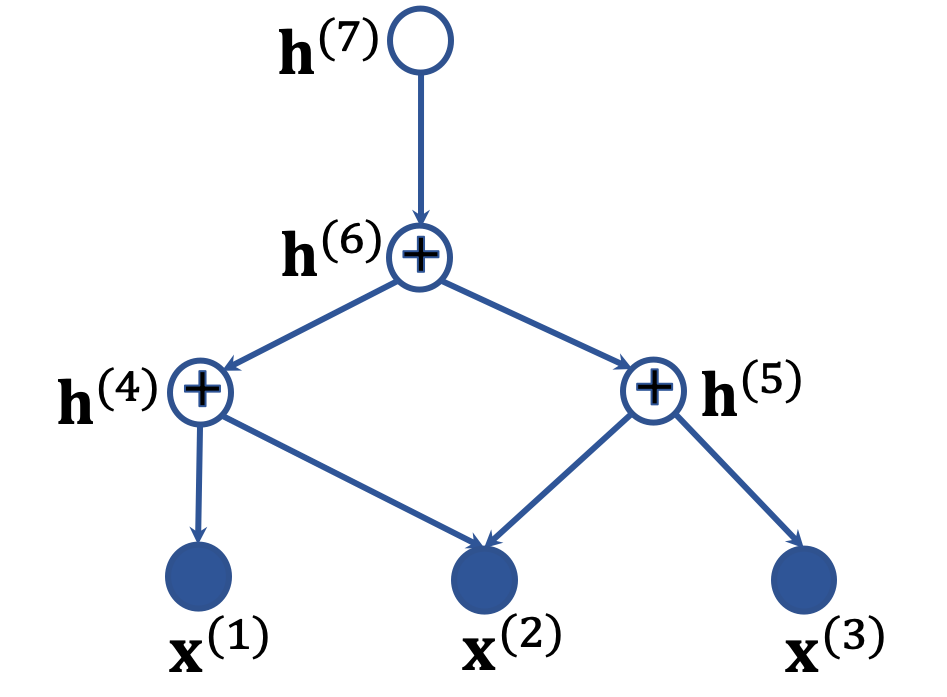
\includegraphics[width=2.3in]{fig/dag.png}
    \caption{DAG structure. The inverse topology order is \big\{ \{1,2,3\}, \{4,5\}, \{6\},  \{7\} \big\}, and it corresponds to layers 0 to 3.  }
    \label{fig:dag}
\end{figure}

Similarly the KL term can be expanded as in the tree structures. For nodes in layer $l$
\begin{align} \label{eq:KL_dag1}
-\text{KL}^{l:L} 
=&     \mathbb{E}_{q(\mathbf{h}^{pa(l)}|\mathbf{h}^l)} \big[  p( \mathbf{h}^{l}|  \mathbf{h}^{pa(l)})    \big]  +  \text{H}_q(\mathbf{h}^{l}|\mathbf{h}^{ch(l)})  - \text{KL}^{l+1:L}.
\end{align}
The forward and backward messages or latent state of a node are stored in the message passing procedures. They can be used by the node's parents and children  to compute the ELBO.  
It enables the calculation even the parents or children are  not  in layer~$l+1$ or $l-1$. For the node $i$ in layer $l$,   $pa(i)$ may have children in layers below $l$. Some nodes in $l$ may not have parent, and combining with the prior, the entropy term will become an KL term in this case.  Thus,  we have 
\begin{align} \label{eq:KL_dag2}
&-\text{KL}^{l:L} \\ \notag
=&   \sum_{i:i\in l, i \not\in   \mathcal{R}_{ \mathcal{G}} }  \bigg\{ \mathbb{E}_{q(\mathbf{h}^{pa(i)}|\mathbf{h}^{ch(pa(i))}} \big[  p( \mathbf{h}^{i}|  \mathbf{h}^{pa(i)})    \big]   +  \text{H}_q(\mathbf{h}^{i}|\mathbf{h}^{ch(i)})  \bigg\}  \\ \notag
& -  \sum_{i \in l \bigcap \mathcal{R}_{ \mathcal{G} }  }  \text{KL}\big(q(\mathbf{h}^{(i)} | \mathbf{h}^{ch(i)} )   | p(\mathbf{h}^{(i)})  \big)  - \text{KL}^{l+1:L}. \notag
\end{align}

By recurrently applying~\eqref{eq:KL_dag2}, we have 
\begin{align} \label{eq:kl_dag3}
& \mathbb{E}_{q(\mathbf{h} | \mathbf{x})} \bigg[ \log  \frac{p( \mathbf{h})}{q(\mathbf{h}|\mathbf{x})}  \bigg] \\ \notag
=& \sum_{l=1}^{L-1}   \sum_{i:i\in l, i \not\in   \mathcal{R}_{ \mathcal{G}}  }  \bigg\{ \mathbb{E}_{q(\mathbf{h}^{pa(i)}|\mathbf{h}^{(i)})} \bigg[ \log p( \mathbf{h}^{(i)}|  \mathbf{h}^{pa(i)})   \bigg]  +    \text{H}(\mathbf{h}^i | \mathbf{h}^{ch(i)} )  \bigg\} \\ \notag
& -   \sum_{l=1}^{L-1}  \sum_{i \in l \bigcap \mathcal{R}_{ \mathcal{G} }  }  \text{KL}\big(q(\mathbf{h}^{(i)} | \mathbf{h}^{ch(i)} )   | p(\mathbf{h}^{(i)})  \big)   -   \text{KL}\big(q(\mathbf{h}^L | \mathbf{h}^{L-1} )   | p(\mathbf{h}^L)  \big) .
 \end{align}
Since $L  \subseteq   \mathcal{R}_{ \mathcal{G}} $,  with $\mathbf{h}^{(0)} = \mathbf{x}$,~\eqref{eq:dag_elbo}, and~\eqref{eq:kl_dag3} we have 
\begin{align*}  
 &\log p(\mathbf{x}) \geqslant  \mathcal{L}(\mathbf{x}; \theta) \\
=&   \sum_{i \in \mathcal{G}  \setminus  \mathcal{R}_{ \mathcal{G} }  }  \mathbb{E}_{q(\mathbf{h}^{pa(i)}|\mathbf{h}^{ch(pa(i))})} \bigg[ \log p( \mathbf{h}^{(i)}|  \mathbf{h}^{pa(i)})   \bigg]  \\
 & +  \sum_{i \in \mathcal{G}  \setminus  \mathcal{R}_{ \mathcal{G} }  } H_q(\mathbf{h}^{(i)} | \mathbf{h}^{ch(i)} )   -    \sum_{i \in  \mathcal{R}_{ \mathcal{G} }  }  \text{KL}\big(q(\mathbf{h}^{(i)} | \mathbf{h}^{ch(i)} )   | p(\mathbf{h}^{(i)})  \big) .   
 \end{align*}

\begin{figure*}[!htbp]%{r{0.4\textwidth}
\begin{center}
 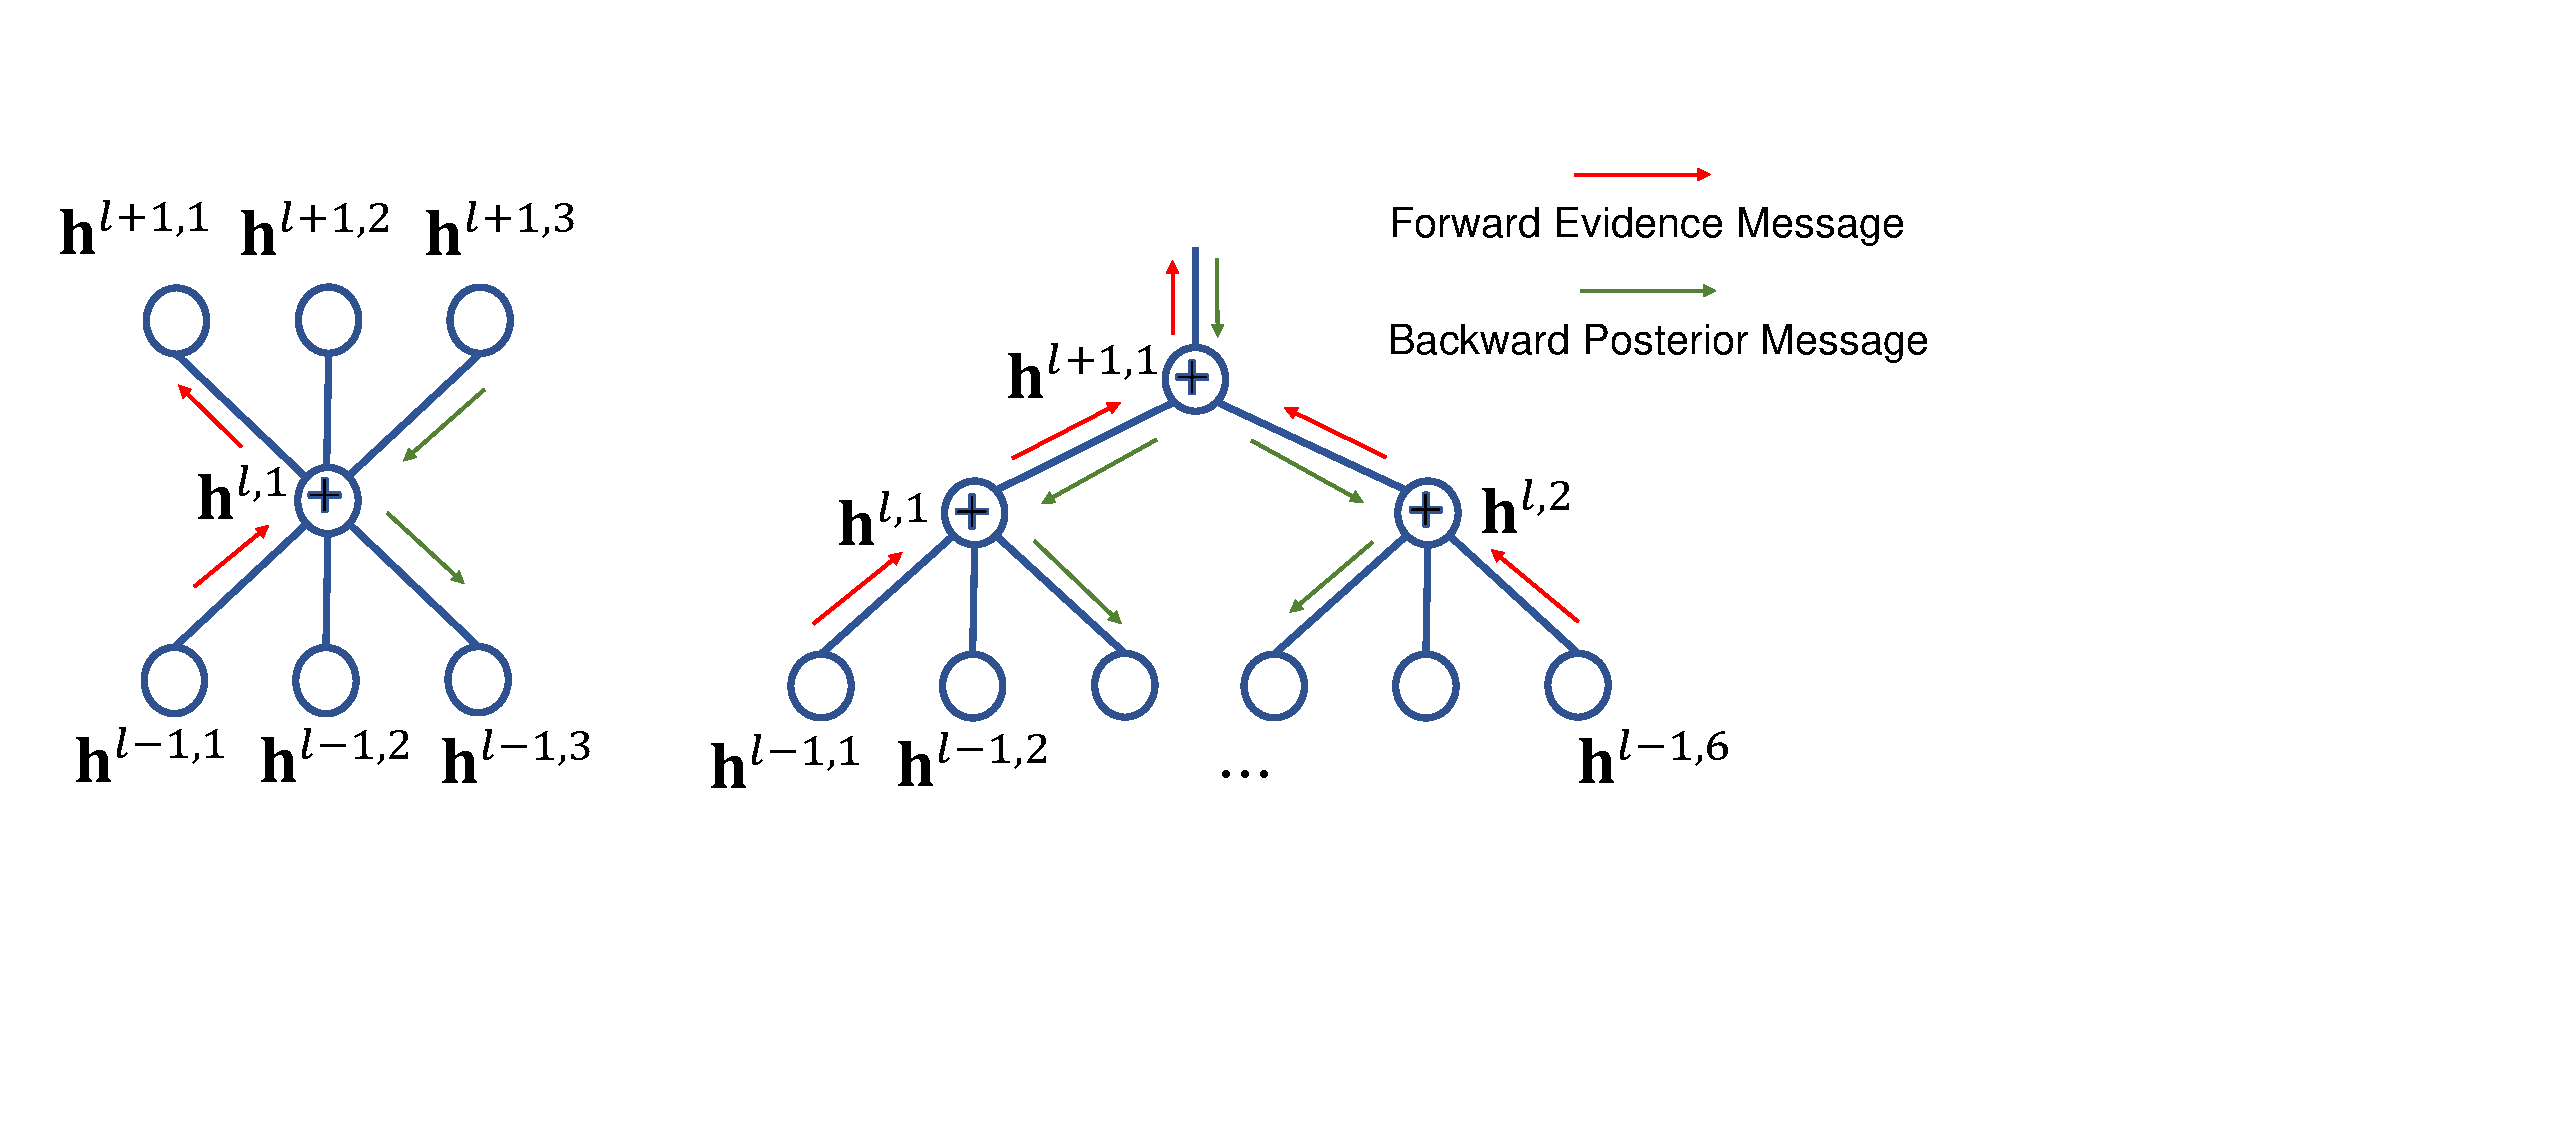
\includegraphics[width=0.7\linewidth]{fig/message_pass.pdf}
\end{center}
  \caption{(Left) Message passing in a node. (Right) Message passing in a tree.} 
\label{fig:message}
\end{figure*}

\section*{Appendix C.  Proof of Lemma1}\label{appd:proof}
Let\textbf{Lemma 1.} {\it Let $\mathcal{G}$ be a well trained tree structured variational flow graphical model with $L$ layers, and $i$ and $j$ are two leaf nodes with $a$ as the closest common ancestor. Given observed value at node $i$, the value of node $j$ can be approximated with   $\widehat{\mathbf{x}}^{j} \approx  \mathbf{f}_{(a,j)}(\mathbf{f}_{(i, a)}(\mathbf{x}^{(i)}))$. Here $\mathbf{f}_{(i, a)}$ is the flow function path from node $i$ to node $a$. The conditional density of $\mathbf{x}^{(j)}$ given $\mathbf{x}^{(i)}$ can be approximated with 
\begin{align*} %\label{eq:cond_llk}
\log p(\mathbf{x}^{(j)} | \mathbf{x}^{(i)}) &\approx  \log p(\widehat{\mathbf{h}}^L) -  \frac{1}{2} \log \big(\det \big(\mathbf{J}_{\widehat{\mathbf{x}}^{(j)}}(\widehat{\mathbf{h}}^L)^\top\mathbf{J}_{\widehat{\mathbf{x}}^{(j)}}(\widehat{\mathbf{h}}^L)\big) \big).
\end{align*}
}
%\end{lemma}


\end{document}